%% All authors must submit their articles at
%% \href{http://www.pnascentral.org/cgi-bin/main.plex}{PNAScentral}. If
%% you are using Overleaf to write your article, you can use the
%% ``Submit to PNAS'' option in the top bar of the editor window.

\documentclass[11pt,twocolumn,twoside,lineno]{pnas-new}
% Use the lineno option to display guide line numbers if required.

\usepackage[utf8]{inputenc}

\templatetype{pnasresearcharticle} % Choose template 
% {pnasresearcharticle} = Template for a two-column research article
% {pnasmathematics} %= Template for a one-column mathematics article
% {pnasinvited} %= Template for a PNAS invited submission

\title{Genotypic variation in a foundation tree alters ecological
  network structure of an associated community}

% Use letters for affiliations, numbers to show equal authorship (if
% applicable) and to indicate the corresponding author

\author[a,b,1]{Matthew K. Lau}
\author[b]{Louis J. Lamit}
\author[c]{Rikke R. Naesbourg}
\author[d]{Stuart R. Borrett}
\author[e]{Matthew A. Bowker}
\author[a]{Thomas G. Whitham}

%% Include department, institution, and complete address, with the
%% ZIP/postal code, for each author. Use lower case letters to match
%% authors with institutions, as shown in the example. 
%% Authors with an ORCID ID may supply this information at submission.

\affil[a]{Department of Biological Sciences and Merriam-Powell Center
  for Environmental Research, Northern Arizona University, Flagstaff,
  AZ 86011, USA}
\affil[b]{Harvard Forest, Harvard University, 324 N Main St,
  Petersham, MA 01366, USA}
\affil[d]{Department of Biology, Syracuse University, 107 College
  Place Syracuse, NY 13244, USA}
\affil[e]{University of California Berkeley, Berkeley, CA, USA}
\affil[f]{Department of Biology and Marine Biology, University of
  North Carolina Wilmington, 601 South College Road, Wilmington, NC,
  28403, USA}
\affil[g]{School of Forestry, Northern Arizona University, Flagstaff,
  AZ 86011, USA}

% Please give the surname of the lead author for the running footer
\leadauthor{Lau} 
% Use letters for affiliations, numbers to show equal authorship (if
% applicable) and to indicate the corresponding author
% Please add here a significance statement to explain the relevance of your work

%% Authors must submit a 120-word maximum statement about the
%% significance of their research paper written at a level
%% understandable to an undergraduate educated scientist outside their
%% field of speciality. The primary goal of the Significance Statement
%% is to explain the relevance of the work in broad context to a broad
%% readership. The Significance Statement appears in the paper itself
%% and is required for all research papers.



\significancestatement{Evolution occurs in the context of ecosystems
  comprised of complex ecological networks. Research at the interface
  of ecology and evolution has primarily focused on pairwise
  interactions among species and have rarely included a genetic
  component to analyses. Here, we use a long-term common garden
  experiment to reveal the effect that genotypic variation can have on
  networks of lichens that occur on the bark of a foundation tree
  species. We found that lichen interaction network structure is
  genetically based and is correlated with heritable bark traits,
  including roughness and condensed tannins. These findings
  demonstrate the importance of genetic variation and evolutionary
  dynamics in shaping ecological networks as evolved traits.}

% Please include corresponding author, author contribution and author
% declaration information

\authorcontributions{M.L. and L.L. conceived the study, M.L. and
  L.L. conducted the field work, R.N.  assisted in lichen
  identifications, M.L. wrote the first draft of the manuscript,
  S.B. and T.W. contributed substantively to the conceptual
  development, T.W. established the common garden. All authors
  contributed to revisions of the manuscript.}
\authordeclaration{The authors have no conflicts of interest.}
\correspondingauthor{\textsuperscript{1}Dr. Matthew K. Lau. E-mail:
  matthewklau@fas.harvard.edu}

% Keywords are not mandatory, but authors are strongly encouraged to
% provide them. If provided, please include two to five keywords,
% separated by the pipe symbol, e.g:
\keywords{networks $|$ heritability $|$ community $|$ genetics $|$
  lichen $|$ cottonwood $|$ Populus $|$ common garden}

\begin{abstract}
%% Please provide an abstract of no more than 250 words in a single
%% paragraph. Abstracts should explain to the general reader the major
%% contributions of the article. References in the abstract must be
%% cited in full within the abstract itself and cited in the text.

%% Currently: 234 words 12November2019

Biological evolution occurs in the context of complex networks of
interacting species in which natural selection defines the structure
of ecological networks. Fundamental to this evolutionary process is
the discovery of a genetic basis to ecological network
structure. Although previous work has demonstrated that tree genotype
contributes to interaction network structure at the scale of forest
stands, the contribution of tree genetics to localized interaction
networks at the scale of individual trees has not yet been
explored. To test the degree to which tree genetics can contribute to
network structure we conducted quantitative modeling of interaction
networks. We constructed networks of epiphytic lichen associated with
individual trees that were a part of a long-term experimental common
garden of genotypes of (\textit{Populus angustifolia}), a foundation
species. We found three main results. First, tree genotype
significantly predicted lichen network similarity, i.e. trees of the
same genotype had more similar lichen networks. Second, bark roughness
and condensed tannin concentration were both predicted by tree
genotype and correlated with lichen network similarity. Third, the
network metrics, the number of links and centrality, were both
correlated with several tree traits, including bark roughness and
condensed tannin concentration. We conclude that tree genotype
influences lichen interaction network structure with two potential
pathways through bark roughness and condensed tannin
concentration. These results provide evidence that variation in
ecological networks can result from genetically based variation in
foundation species.


\end{abstract}

\dates{This manuscript was compiled on \today}
\doi{\url{www.pnas.org/cgi/doi/10.1073/pnas.XXXXXXXXXX}}

\begin{document}

%% Many authors find it useful to organize their manuscripts with the
%% following order of sections; Title, Author Affiliation, Keywords,
%% Abstract, Significance Statement, Results, Discussion, Materials
%% and methods, Acknowledgments, and References. Other orders and
%% headings are permitted.

%% PNAS generally uses a two-column format averaging 67 characters,
%% including spaces, per line. The maximum length of a Direct
%% Submission research article is six pages and a Direct Submission
%% Plus research article is ten pages including all text, spaces, and
%% the number of characters displaced by figures, tables, and
%% equations.  When submitting tables, figures, and/or equations in
%% addition to text, keep the text for your manuscript under 39,000
%% characters (including spaces) for Direct Submissions and 72,000
%% characters (including spaces) for Direct Submission Plus.

%% Authors may use 1- or 2-column equations in their article,
%% according to their preference.

%% To allow an equation to span both columns, use the
%% \verb|\begin{figure*}...\end{figure*}| environment mentioned above
%% for figures.

%% Note that the use of the \verb|widetext| environment for equations
%% is not recommended, and should not be used.

%% \begin{figure*}[bt!]
%% \begin{align*}
%% (x+y)^3&=(x+y)(x+y)^2\\
%%        &=(x+y)(x^2+2xy+y^2) \numberthis \label{eqn:example} \\
%%        &=x^3+3x^2y+3xy^3+x^3. 
%% \end{align*}
%% \end{figure*}


%% \begin{table}%[tbhp]
%% \centering
%% \caption{Comparison of the fitted potential energy surfaces and ab
%% initio benchmark electronic energy calculations}
%% \begin{tabular}{lrrr}
%% Species & CBS & CV & G3 \\
%% \midrule
%% 1. Acetaldehyde & 0.0 & 0.0 & 0.0 \\
%% 2. Vinyl alcohol & 9.1 & 9.6 & 13.5 \\
%% 3. Hydroxyethylidene & 50.8 & 51.2 & 54.0\\
%% \bottomrule
%% \end{tabular}
%% \addtabletext{nomenclature for the TSs refers to the numbered
%% species in the table.}
%% \end{table}

%% References should be cited in numerical order as they appear in
%% text; this will be done automatically via bibtex,
%% e.g. \cite{belkin2002using} and
%% \cite{berard1994embedding,coifman2005geometric}. All references
%% should be included in the main manuscript file.

%% PNAS must be able to archive the data essential to a published
%% article. Where such archiving is not possible, deposition of data
%% in public databases, such as GenBank, ArrayExpress, Protein Data
%% Bank, Unidata, and others outlined in the Information for Authors,
%% is acceptable.


%% Only TIFF, EPS, and high-resolution PDF for Mac or PC are allowed
%% for figures that will appear in the main text, and images must be
%% final size. Authors may submit U3D or PRC files for 3D images;
%% these must be accompanied by 2D representations in TIFF, EPS, or
%% high-resolution PDF format.  Color images must be in RGB (red,
%% green, blue) mode. Include the font files for any text.

%% Figures and Tables should be labeled and referenced in the
%% standard way using the \verb|\label{}| and \verb|\ref{}| commands.

%% Figure \ref{fig:frog} shows an example of how to insert a
%% column-wide figure. To insert a figure wider than one column,
%% please use the \verb|\begin{figure*}...\end{figure*}|
%% environment. Figures wider than one column should be sized to 11.4
%% cm or 17.8 cm wide. Use \verb|\begin{SCfigure*}...\end{SCfigure*}|
%% for a wide figure with side captions.

%% Authors should submit SI as a single separate PDF file, combining
%% all text, figures, tables, movie legends, and SI references.  PNAS
%% will publish SI uncomposed, as the authors have provided it.
%% Additional details can be found here:
%% \href{http://www.pnas.org/page/authors/journal-policies}{policy on
%% SI}.  For SI formatting instructions click
%% \href{https://www.pnascentral.org/cgi-bin/main.plex?form_type=display_auth_si_instructions}{here}.
%% The PNAS Overleaf SI template can be found
%% \href{https://www.overleaf.com/latex/templates/pnas-template-for-supplementary-information/wqfsfqwdiscujtsd}{here}.
%% Refer to the SI Appendix in the manuscript at an appropriate point
%% in the text. Number supporting figures and tables starting with S1,
%% S2, etc.

%% Authors who place detailed materials and methods in an SI Appendix
%% must provide sufficient detail in the main text methods to enable a
%% reader to follow the logic of the procedures and results and also
%% must reference the SI methods. If a paper is fundamentally a study
%% of a new method or technique, then the methods must be described
%% completely in the main text.


\maketitle \thispagestyle{firststyle}
\ifthenelse{\boolean{shortarticle}}{\ifthenelse{\boolean{singlecolumn}}{\abscontentformatted}{\abscontent}}{}

% If your first paragraph (i.e. with the \dropcap) contains a list
% environment (quote, quotation, theorem, definition, enumerate,
% itemize...), the line after the list may have some extra
% indentation. If this is the case, add \parshape=0 to the end of the
% list environment.

%% \dropcap{T}his PNAS journal template is provided to help you write
%% your work in the correct journal format.  Instructions for use are
%% provided below.

%% Note: please start your introduction without including the word
%% ``Introduction'' as a section heading (except for math articles in
%% the Physical Sciences section); this heading is implied in the
%% first paragraphs.

%% Introduction

%% - Evolution occurs in complex ecological networks, which have been
%% treated primarily from a pairwise perspective
%% - Network ecology suggests that network architecture has important
%% implications for ecological and evolutionary dynamics
%% - Community genetics has shown that intraspecific variation impacts
%% communities and ecosystems
%% - What we know about networks in a community genetics context is
%% Bailey 2009 (tri-trophic chain), Bridgeland ????, Smith 2012
%% (geographic mosaic), Lamit 2015 (JoE), Lau 2016 (bipartite), Keith
%% 2017 (bipartite).
%% - None of these studies have looked at networks of organisms at a
%% scale in which population genetics of trees might impact entire
%% networks of interacting organisms, hence this study
%% - Hypothesis: based on the genetic similarity rule, genetically
%% similar individuals should tend to have similar communities and
%% based on past research with network ecology, they should also have
%% similar interaction networks

\begin{itemize}
\item Evolution occurs in complex ecosystems
\item Community genetics studies have demonstrated the importance of
genetics and evolutionary dynamics in structuring communities and
ecosystems
\item Community composition, ecosystem processes have been shown to vary
in response to the genetic variation of foundation species
\item Previous studies have examined aspects of networks but to date, no
studies have examined the genetic basis of networks of interacting
species
\item Here we examine the genetic basis of network structure on a
community of sessile lignicolous (i.e. bark) lichen on cottonwood
trees. This system is ideal for examining for this kind of study
because it:

\begin{enumerate}
\item Lichen do not move among trees, although asexual propagules could
  move to other trees in the garden 
\item Is not unapproachably complex
\item Is comprised of distinct individuals that are small enough for an
  entire community to occur on a single tree but not too small to be
  quantified easily
\end{enumerate}

\item We hypothesize that trees will vary in some phenotypic traits, such
that trees of the same genotype will tend to have similar traits
producing similarities in lichen network structure. To test this
hypothesis, we use a common garden of cottonwood trees with lichen
communities.
\end{itemize}


\dropcap{E}volution occurs in the context of complex ecological
networks. Initially, evolution in a community context was focused on
examples of highly co-evolved pairs of species (e.g. Darwin's famous
prediction of the Sphinx Moth and Christmas Orchid)
cite{Wade2007}. However, studies of diffuse co-evolution
(\textit{sensu} cite{Janzen1980}) cite{Stinchcombe2002, Strauss2007,
  Dicke2010}, geographic mosaics of co-evolution cite{Thompson2005}
and community genetics cite{Whitham2006} have provided an in-road for
ecological network approaches cite{Fortuna2009, Keith2017, Lau2016} to
illuminate a more complex perspective of the interface between
ecological and evolutionary dynamics. There is now evidence to support
that selection tends to occur among groups of species cite{Wade2007,
  Pieterse2007, Dicke2010} favoring the development of small webs
cite{Nuismer2006, Guimaraes2007, Gomez2009} and that genetic variation
and phylogenetic relatedness contributes to variation in community
assembly \cite{Crutsinger2016} and species interactions
cite{Whitham2006a, Bailey2009, Moya-Larano2011}, which shapes the
ecological interaction networks \cite{Rezende2007}. 

Community genetics studies \cite{Lamit2015a} have shown that genetic
variation in foundation species \cite{Ellison2005} plays a significant
role in defining distinct communities of interacting organisms:  such
as, endophytes, pathogens, lichens, arthropods, and soil
microbes. Multiple studies have now demonstrated that genetic
variation influences numerous functional traits (e.g., phytochemical,
phenological, morphological) produces a multivariate phenotype
\cite{holeski2012} that contributes to variation in associated
communities \cite{Bailey2009a}. The importance of genetic variation in
structuring ecological systems was recently reviewed by Des Roches et
al. (2018). 

Additional work has provided support for the hypothesis that not only
does composition vary among genetically distinct genotypes of
foundation species, it also impacts the structure of the network of
species interactions in these communities. Two studies have
demonstrated conceptually \cite{Lau2015a} and empirically
\cite{Keith2017}. However, studies in the network ecology literature
generally do not include a genetic component (see review by Borrett et
al. 2014) and community genetics papers do not have data on network
structure of associated communities. Currently, we are aware of only
one paper that empirically examines the genetic basis of network
structure of a community cite{Barbour2019}.


Here, we investigate how genetic variation in a foundation tree
species determines the structure of a network of interactions among a
community of tree associated lichen species. Using a long-term (20+
years), common garden experiment with replicated individuals of known
genetic identity and a naturally established stand of \textit{Populus
  angustifolia}. We focused on a model community of 9 epiphytic lichen
species, as previous research has demonstrated significant
compositional responses of epiphytes to genotypic variation
\cite{Winfree2011, Zytynska2011}. In addition, the life-history
characteristics of lichens, having highly localized, direct contact
interactions and slow population turnover rates, allowed us to assess
interactions among lichen species on individual trees. We hypothesize
that in natural systems evolution occurs in a community context
involving interactions of complex networks of interacting species
\cite{Lau2015a, Keith2017, Thompson2013, Bascompte2006}.  If correct,
we expect to find that network structure is genetically based in which
different plant genotypes support different interaction networks and
that these interactions networks can function as indicators of
ecological dynamics important for conserving biodiversity.  Applying a
probability-theory based network modeling approach, we constructed a
set of interaction network models for the lichens associated with
individual trees. Using these models, we then examined the genetic
basis of the structure of these ecological networks.




\matmethods{

The study was conducted along the Weber River, UT (USA), which is a
cottonwood (\textit{Populus} spp.) dominated riparian
ecosystem. Although two native species, \textit{Populus angustifolia}
(James) and \textit{Populus fremontii} (S. Watson), occur here and are
known to hybridize, only pure or advanced generation backcrosses of
\textit{P. angustifolia} were sampled. Bark lichens have been
extensively studied in this system and provide an ideal system in
which to observe and model lichen interaction networks, as their
sessile nature permits accurate identification of individuals
\cite{Lamit2011}.

A long-term, common garden experiment was used to isolate the effect
of tree genotype from the effect of the localized microenvironment
associated with each individual and spatial
autocorrelation. Established in 1992, asexually propagated clones of
genotyped \textit{P. angustifolia} individuals were obtained from wild
collections and planted in fully randomized design at the Ogden Nature
Center, Ogden, UT. From the population of established individuals in
the common garden, we chose a total of thirteen genotypes, replicated
between 3 and 8 times each, for sampling.


\subsection*{Bark Lichen Observations}


On each tree, presence or absence of each lichen species was assessed
in 50 total 1 cm$^2$ cells arrayed in a checkerboard pattern. Given
the small size and sessile nature of lichens, we were able to rapidly
assess lichen interactions by quantifying thalli in close
contact. Sampling was restricted to the northern aspect of the trunk
to maximize the abundance of lichen and control for the effect of
trunk aspect. Two adjacent 10 cm$^2$ quadrats centered at 50 cm and 85
cm from ground level were sampled (Fig~\ref{fig:lichen_sampling} A and
B). The observed lichen community included (abbreviations are given
for species present in study): Xg = \textit{Xanthomendoza
  galericulata}, Xm = \textit{X. montana}, Ch = \textit{Caloplaca
  holocarpa}, Cs = \textit{Candelariella subdeflexa}, Rg =
\textit{Rinodina glauca}, Lh = \textit{Lecanora hagenii}, Pm =
\textit{Phyciella melanchra}, Pa = \textit{Physcia adscendens}, Pu =
\textit{Physcia undulata}. Several other species were not obesrved in
the present study but are known to occur in this region:
\textit{Phaeophyscia orbicularis}, \textit{Phaeophyscia ciliata},
\textit{Melanelia subolivacea}, \textit{Meanelia elegantula}.


The cell size and checkerboard sampling pattern was chosen to isolate
the individuals in each cell. In a previous survey of lichen thallus
size in this common garden, we had observed a median thallus size of
0.12 $\pm$ 0.001 cm$^2$ (1 S.E.) (see Supporting Information). Based
on the median thallus size, we expected thalli observed in each cell
to generally be spatially independent of thalli present in other cells
but exposed to similar micro-environmental conditions created by the
bark and the location of the sampling area on an individual
tree. Therefore, we were confident in treating the cell-wise
observations in quadrats as independent with respect to lichen-lichen
interactions.


We also measured several bark traits for each tree: including, bark
roughness and chemistry. \textbf{INSERT FROM LAMIT}.



\begin{figure*}[ht]
\centering
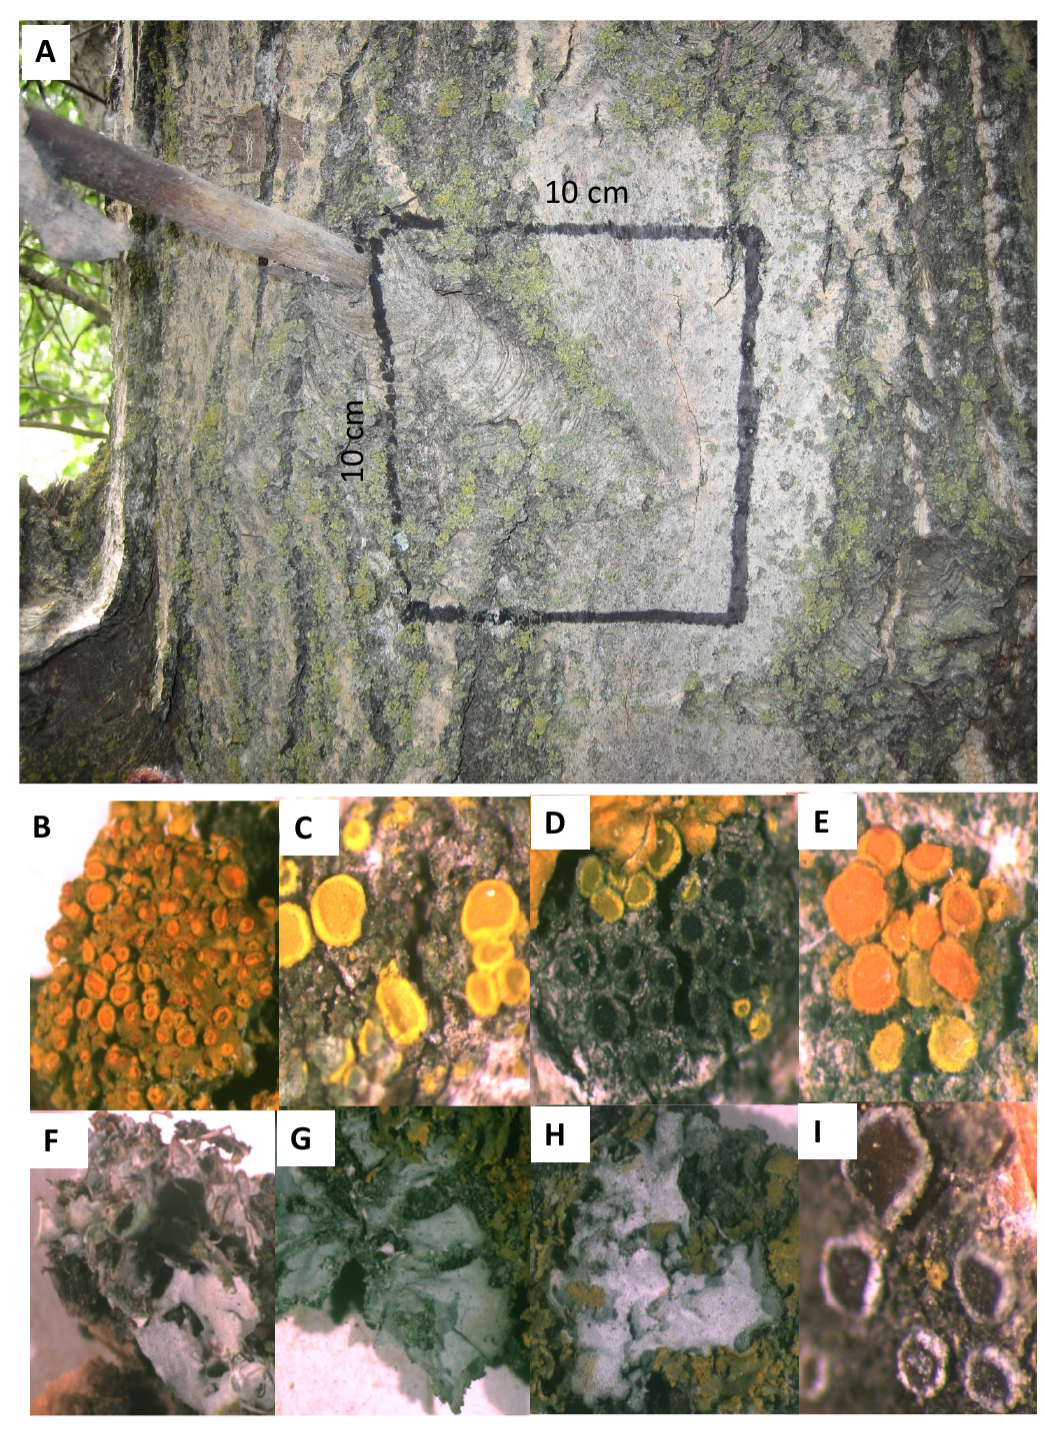
\includegraphics[width=\linewidth]{lcn_sampling.pdf}
\caption{The communities of bark lichens were observed in a common
  garden of replicated genotypes of narrowleaf cottonwood trees
  (\textit{P. angustifolia}) at the Ogden Nature Center (Ogden,
  UT). Lichens were sampled within a fixed area (10 cm$^2$) on
  individual trees at two heights, 40cm and 80cm from the ground (A
  and B, respectively). (C) a photo of a typical community of bark
  lichen species interacting on the trunk of a cottonwood tree,
  including one of the more abundant species, \textit{Xanthomendoza
    galericulata}, in the center. (D-K) shows the other lichen species
  observed, respectively:  \textit{X. montana}, \textit{Candelariella
    subdeflexa}, \textit{Rinodina} sp., \textit{Caloplaca holocarpa},
  \textit{Physcia adscendens}, \textit{Phyciella melanchra},
  \textit{Physcia undulata} and \textit{Lecanora hagenii}. Photo
  Credits: L.J. Lamit (A-C) and R.R. Naesbourg (D-K).}
\label{fig:lichen_sampling}
\end{figure*}


\subsection*{Lichen Network Modeling and Analysis}

For each tree, repeated observations of lichen were made in order to
construct replicated interaction networks for each genotype. We
quantified the presence of lichen in the 1 cm$^2$ cells on individual
trees of \textit{P. angustifolia}. Unipartite networks were generated
using the conditional probabilities of each species pair, i.e. the
probability of observing one species given an observation of another
species $P(S_i | S_j)$, based on the method developed by
\citep{Araujo2011}. To calculate conditional probabilities, we
quantified the individual probabilities of species occurrences
$P(S_i)$ and the joint probability of co-occurrences $P(S_i,S_j)$
using the frequencies of each species and their co-occurrences. We
were then able to calculate the conditional probabilities of each
species pair as $P(S_i|S_j) = \frac{P(S_i,S_j)}{P(S_j)}$, based on the
axioms of probability. This yielded a matrix that could possibly be
asymetric, i.e. $P(S_i|S_j)$ does not have to be equal to
$P(S_j|S_i)$. Another important property of this matrix is that the
diagonal ($S_{ii}$) was equal to one for all species present and zero
for species that were not observed in any cell.

We then applied an analytical procedure to remove non-significant
links between species. This procedure determines if the joint
probability of a species pair (i.e. $P(S_i,S_j)$) is different from
zero (Fig.~\ref{fig:conet_method}).  Here, a confidence interval
$CI_{95\%}$ is calculated as as $CI_{95\%} = E[S_iS_j] * Z_{95\%} *
\sqrt{V(S_iS_j)}$, where the expected frequency of co-occurrences
E($S_iS_j$) is the total number of cells surveyed ($N$) times the
independent probabilities of each species $P(S_i) * P(S_j)$,
$Z_{95\%}$ is the Z-score for 95\% from a Z-distribution and the
expected variance of $E(S_iS_j)$ is the total number of cells times
the expected probability of $S_iS_j$ and its compliment
(i.e. $V(S_iS_j) = N * E[P(S_i,S_j)] * (1 - E[P(S_i,S_j)])$). If the
observed number of co-occurrence falls outside of the confidence
interval, the joint probability $P(S_i,S_j)$ is determined to be equal
to the product of the individual probabilities (i.e. $P(S_i) \dot
P(S_j)$), and the conditional probability reduces to the individual
probability of that species $P(S_i)$. Therefore, unless the
co-occurrence of a species pair falls outside the confidence interval,
the probability that the observation of one species given the other is
no different than simply observing that species alone. This enables us
to remove links from a given network by re-scaling the resulting
conditional probabilities by subtracting the individual probabilities
from the conditional probabilities (i.e. how different the conditional
probability is from the independent probability), which makes any
species with a non-significant conditional probability zero. The
resulting matrix ($\mathbf{D} = D_{ij}$) can be interpreted as how one
species impacts another with zero being no effect and values less than
or greater than zero interpreted as negative and positive effects,
respectively. Here, we will refer to this matrix ($\mathbf{D}$) as an
interaction matrix with the properties that it can be asymetric
(i.e. $P_{ij}$ does not necessarily equal $P_{ji}$), and the diagonal
($P_{ii}$) is zero (i.e. a species does not influence it's own
probability of being observed).

\begin{figure*}[ht]
\centering
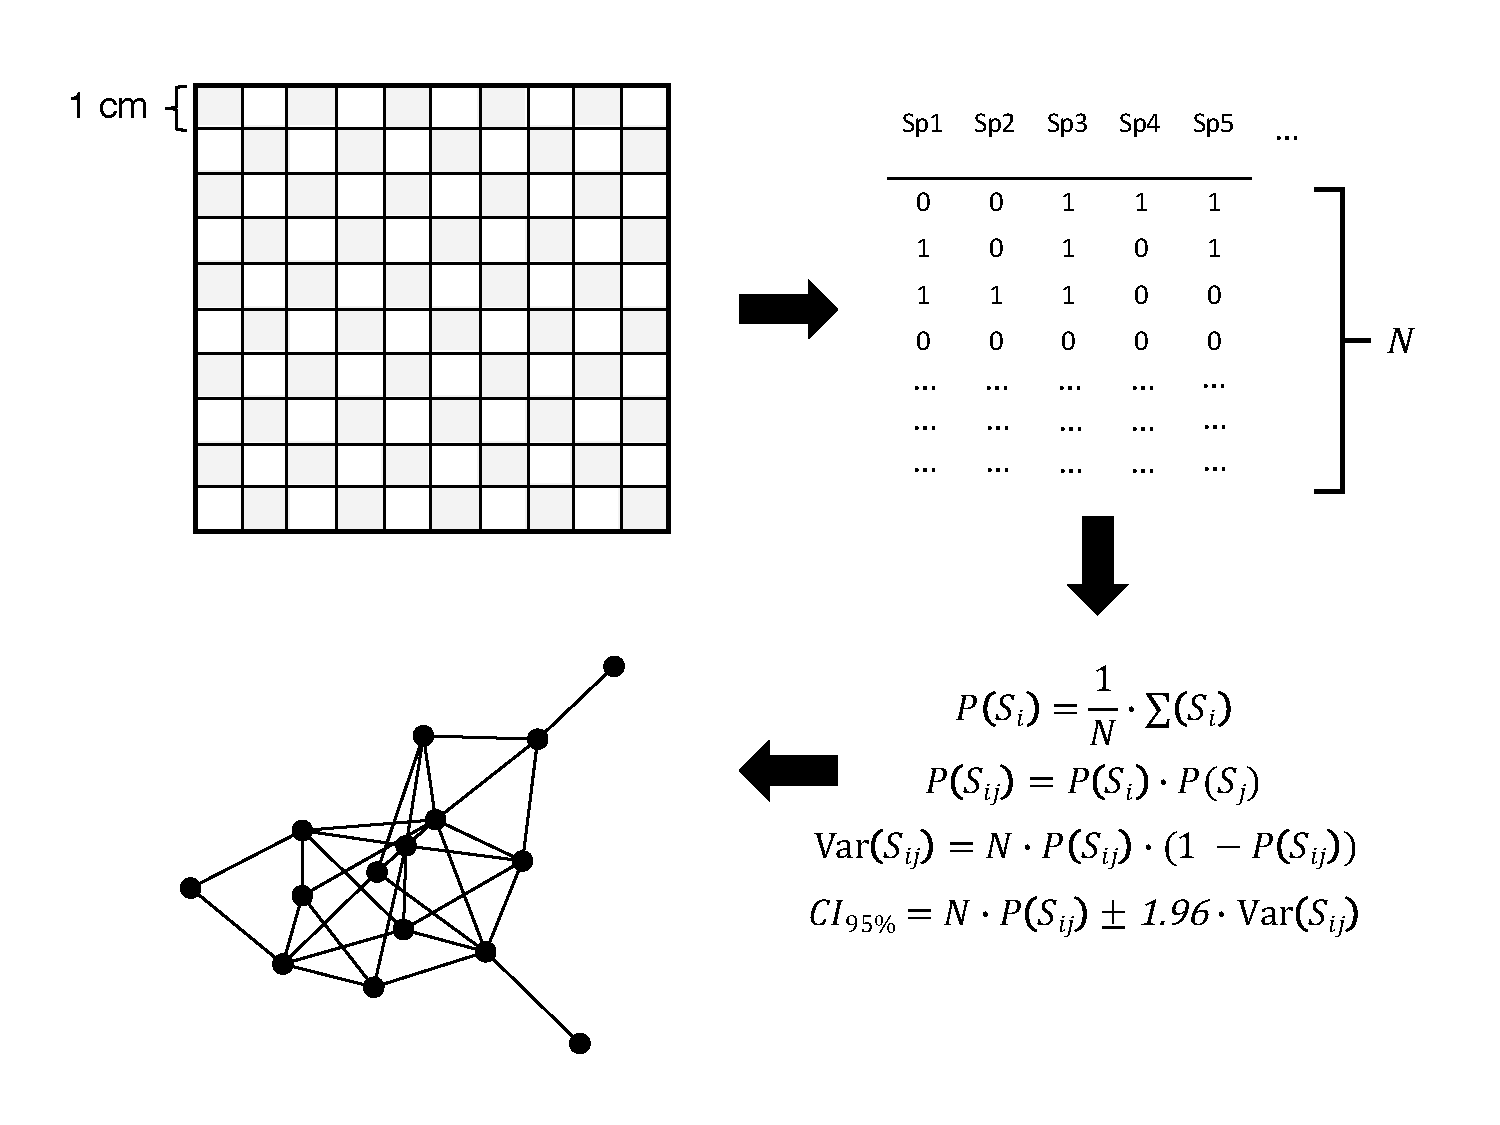
\includegraphics[width=\linewidth]{lcn_araujo_method.pdf}
\caption{Lichen interaction networks were constructed by conducting
  field observations in 1 cm$^2$ cells within a 10 cm$^2$ grid on each
  tree using a checkerboard pattern (grey cells). Thus, a set of $N$
  total cell observations were recorded for each tree with the
  presence or absence of each species recorded for each cell. Applying
  the probability-based network modeling method adapted from
  \cite{Araujo2011}, we calculated the conditional probabilities,
  $P(S_i|S_j)$, for all species pairs and removed (i.e. set equal to
  zero) species pairs whose joint probabilities, $P(S_i S_j)$, were
  not significant using a confidence interval based comparison of
  their observed co-occurrence frequency, $S_iS_j$, to that expected
  due to chance alone, $E[P(S_iS_j)] = P(S_i) P(S_j)$, and
  $P(S_i|S_j)$ reduces to $P(S_i)$, the observed individual
  probability of species $S_i$.}
\label{fig:conet_method}
\end{figure*}



\subsection*{Statistical Analyses, Software and Data}

We used a combination of parametric and non-parametric, permutation
based frequentist statistical analyses to test for the effects of
genetic variation on lichen communities and their interaction
networks. To assess the effect of genotype on univariate responses, we
used additive, random effects models with Restricted Maximum
Likelihood (REML). We used a combination of Least Squares Regression,
Analysis of Variance (ANOVA) and correlation tests to quantify and
test for the relationship among other variables. Bark roughness,
lichen cover and species richness were square-root transformed to meet
the assumptions of homogeneity of variance and normality for these
tests.

For multivariate response variables, such as lichen community
composition and network structure, we used distance based multivariate
statistical approaches, including Permutational Analysis of Variance
(PERMANOVA) and Mantel tests. For some analyses, community composition
was relativized by species maxima to reduce the effect of the highly
abundant \textit{X. galericulata}. For community composition we used
Bray-Curtis dissimilarity, which has optimal performance with count
data citep{Minchen1998}. To quantify the similarity of lichen
networks among individual trees, we calculated the pairwise Euclidean
distance of the $\mathbf{D}$ interaction matrices among all pairs of
trees.

For visualization of multivariate patterns, we used Non-metric
Multi-Dimensional Scaling (NMDS) cite{ecodist} to produce
dimensionally reduced ordinations of these multi-variate responses and
fitted vectors for continuous predictor variables to the ordinated
values cite{vegan}. Using random initial configurations with a
maximum of 500 iterations and a change in stress threshold of less
than 10$^{-12}$. Final configurations has the lowest stress with at
most a stress level of 0.10.


For each network, we also calculated metrics that measure different
structural aspects. Although there are many other metrics, for the
sake of simplicity we focus on a subset that represent several
interesting features of network structure (see \citep{Lau2017a}). We
calculated the number of interactions or ``links'' in each network,
which provides a measure of the size of the network citep{Lau2015,
  Borrett2014}. We also calculated the centralization of each network,
which measures the evenness of the distribution of interactions among
the species in the network cite{Butts2005}. In a network with a low
level of centralization species have similar amount of interaction in
the network, while a network with a high level of centralization tends
to have one or small number of species that interact with other
species. We used a related function to calculate the centrality of
each species (i.e. node level centrality) in each network as well. The
modularity of each network was also quantified using a weighted
algorithm cite{Beckett2016}, which measures the degree to which a
given network is divided into groups of species more connected to each
other than other species. As with the other response variables, the
number of links was log-transformed and both modularity and
centralization scores were fourth-root transformed to meet variance
and normality assumptions.

All code and data for the project are openly available online. Code
and data are available at \url{github.com/ecgen/comgen}. The project
is also archived via Zenodo at \url{zenodo.com/doiXXXXXX}. All
analyses were conducted using the programming language R version 3.6.1
(R Development Core Team 2019).

\begin{figure}[ht]
\centering
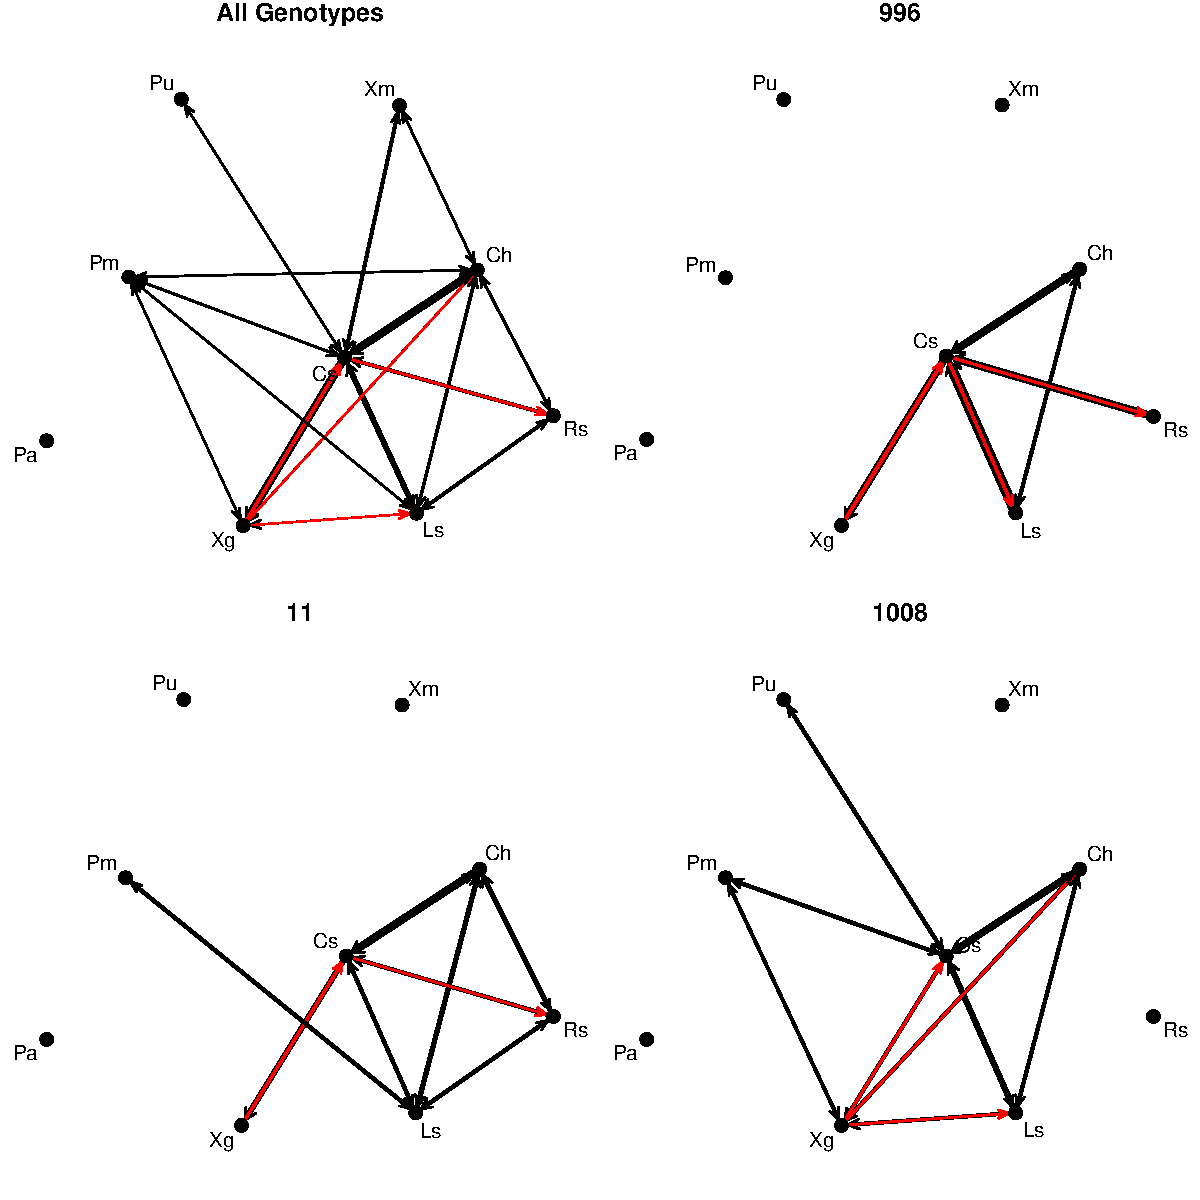
\includegraphics[width=\linewidth]{cn_onc.pdf}
\caption{Lichen networks varied in structure among tree
  genotypes. Network diagrams of the mean lichen interaction matrices
  averaged for all trees and for several individual genotypes showing
  a range of interaction network structure. Directionality
  (arrowheads) and sign (red = negative, black = positive) of
  interactions are shown as edges between species (abbreviated by the
  first letter of the genus and specific epithet), which are scaled by
  their magnitude. The sign of the interaction is indicative of
  greater (positive) or lesser (negative) paired occurrences than
  expected relative to the overall frequency of occurrence of each
  species. Ecologically, the links in the network are likely the
  product of multiple types of interactions (e.g. mutualism,
  parasatism, competition, facilitation) that could vary over both
  space and time.}
\label{fig:geno_nets}
\end{figure}
}

\showmatmethods{} % Display the Materials and Methods section

\section*{Results}


%% New results Fri May  1 19:00:26 EDT 2020

\begin{enumerate}
\item Genotype influenced lichen network structure
  \begin{itemize}
   \item Tree genotype significantly predicted the similarity of
     lichen networks (Pseudo-$F_{9,27}$ = 3.58, $H^2$ = 0.41, \textit{p-value} = 0.0537). 
   \item All network metrics examined responded signficantly to tree
     genotype: including the number of links (\textit{RLRT} = ?, $H^2$
     = 0.32, \textit{p-value} = 0.0269), AMI (\textit{RLRT} = ?, $H^2$
     = 0.31, \textit{p-value} = 0.0268) and degree centralization
     (\textit{RLRT} = ?, $H^2$ = 0.33, \textit{p-value} = 0.0196).
   \item Fig 1. NMDS crosshair with vectors
   \item Supplementary Table. Vectors
   \item Supplementary Table. h2-net
  \end{itemize}
\item Genotype impacts were on positive interactions mainly driven by Ch
  \begin{itemize}
  \item Tree genotype significantly predicted both in-degree
    (\textit{RLRT} = ?, $H^2$ = 0.35, \textit{p-value} = 0.0157) and
    out-degree (\textit{RLRT} = ?, $H^2$ = 0.33, \textit{p-value}
    = 0.0195) centralization.
  \item \textit{Caloplaca holocarpa} centrality was the only species
    to exhibit a significant response to tree genotype (\textit{RLRT}
    = ?, $H^2$ = ?, \textit{p-value} = ?).
  \item Fig 2. dot plot centralization in/out pos/neg
  \item REFER table: h2-net
  \item Supplementary Table: species centrality
  \end{itemize}
\item Genotype indirectly influenced lichen network centralization via bark roughness
  \begin{itemize}
   \item BR ~ Geno (REML), but not other traits (\textit{RLRT} = ?,
     $H^2$ = 0.32,\textit{p-value} = 0.0128)
   \item Net ~ BR (PERMANOVA) ($F_{1,32}$ = 13.029, $R^2$ = 0.26,
     \textit{p-value} = 0.0096)
   \item Centrality was significantly correlated with bark roughness
     ($F_{1, 32}$ = ?, $R^2$ = ?, \textit{p-value} = ?)
   \item However, tree genotype did not significantly predict the
     variation in the residuals from the regression of centrality and
     bark roughness (\textit{RLRT} = ?, $H^2$ = 0.011, \textit{p-value} = 0.4219)
   \item Fig. cross-hair plot Cen ~ BR with trend line
   \item Table: h2_trait.tex
   \item Supplementary Table: cn-trait-perm.tex
   \item Supplementary Table: geno-trait-path.tex
  \end{itemize}
\item Net(sim) ~ Other lichen variation (LM) not genetically based (PERMANOVA)
\end{enumerate}

%% OLD results

Network similarity and several tree traits were genetically
based. Tree genotype was a significant predictor of network similarity
(H$^2$ = 0.16, \textit{p-value} $\leq$ 0.001). Bark roughness (H$^2$ =
0.38, \textit{p-value} $\leq$ 0.001) and condensed tannin
concentration (H$^2$ = 0.28, \textit{p-value} = 0.014) also showed a
signature of tree genotype (Fig.~\ref{fig:h2_plot}); however, this was
not the case for other tree traits, bark pH and carbon to nitrogen
ratio. Also, none of the lichen network metrics were significantly
predicted by tree genotype, either at the scale of the entire network
(Table~\ref{tab:h2_net}) or for individual species (see Supporting
Information). Although both showed a response to tree genotype, bark
roughness and condensed tannins were not correlated (Pearson's $r$ =
0.084, \textit{p-value} = 0.556).

% Table: H2 table
% latex table generated in R 3.6.3 by xtable 1.8-4 package
% Thu May 14 16:39:05 2020
\begin{table}[ht]
\centering
\begin{tabular}{rrrr}
  \hline
response & statistic & H2 & p-value \\ 
  \hline
Lichen Network Similarity & 3.5821 & 0.4130 & 0.0537 \\ 
  Centralization & 4.0444 & 0.3305 & 0.0184 \\ 
  Centralization In-Degree & 4.4812 & 0.3487 & 0.0142 \\ 
  Centralization In-Degree (positive) & 3.9852 & 0.3309 & 0.0190 \\ 
  Centralization In-Degree (negative) & 0.3304 & 0.1057 & 0.2508 \\ 
  Centralization Out-Degree & 3.8615 & 0.3193 & 0.0205 \\ 
  Centralization Out-Degree (positive) & 3.5585 & 0.3119 & 0.0248 \\ 
  Centralization Out-Degree (negative) & 0.0862 & 0.0513 & 0.3446 \\ 
  Number of Network Links (Degree) & 3.5175 & 0.3156 & 0.0255 \\ 
  Degree (positive) & 3.6925 & 0.3242 & 0.0229 \\ 
  Degree (negative) & 0.0327 & 0.0318 & 0.3859 \\ 
   \hline
\end{tabular}
\caption{Genotypic effects on the associated lichen network structure.} 
\label{tab:h2_net}
\end{table}


\begin{figure*}[ht]
\centering
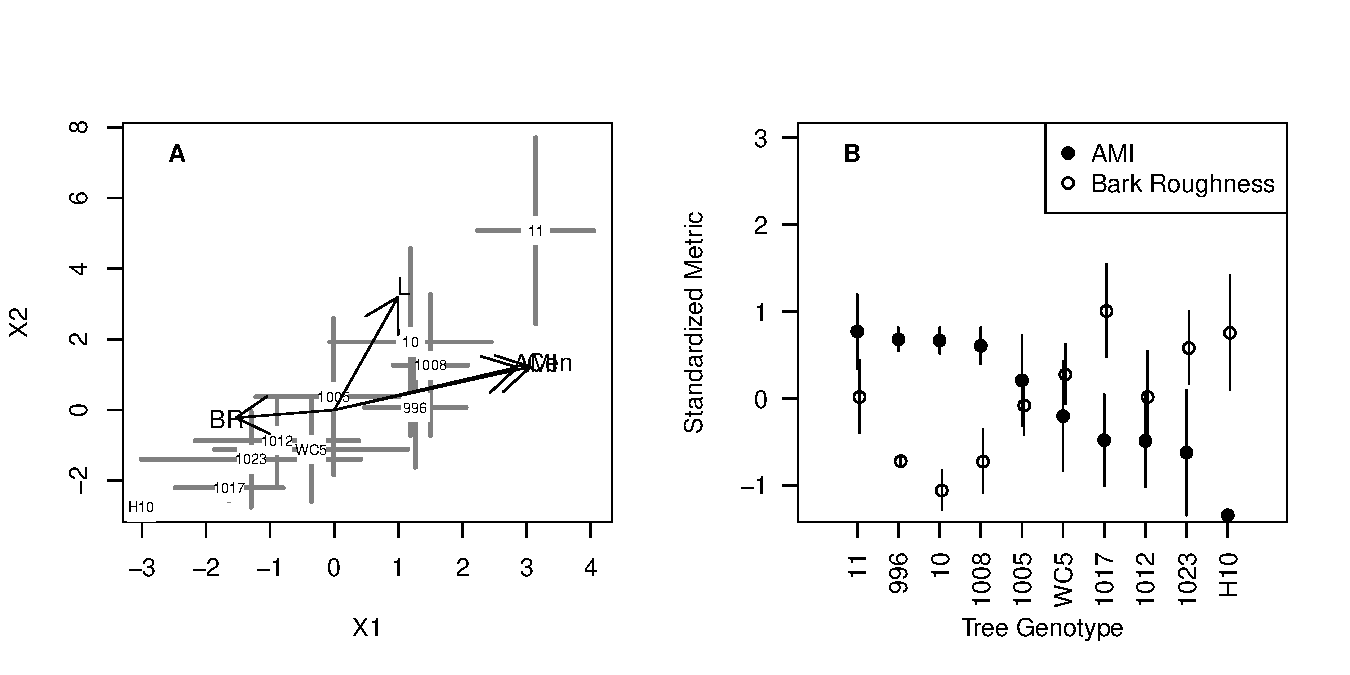
\includegraphics[width=\linewidth]{h2_plot.pdf}
\caption{Tree genotype affected lichen networks and several bark
  traits. A. The plot shows genotype centroids of NMDS ordinated
  (R$^2$ = 0.999, stress = 0.008) lichen networks ($\pm$ 1
  S.E.). Centroids that are closer are more similar in the structure
  of their lichen networks.  B. Plot showing the standardized
  ($\frac{x - \bar{x}}{\sigma}$) means ($\pm$ 1 S.E.) for the two
  genetically based tree traits: tree bark roughness and condensed
  tannin concentration.}
\label{fig:h2_plot}
\end{figure*}

Tree traits and lichen community metrics were correlated with lichen
networks. The genetically based traits, bark roughness and condensed
tannins were both significant predictors of network similarity
(Table~\ref{tab:cn_perm}). Bark C:N ratio was also a significant
predictor of network similarity, but, as shown previously (see
Table~\ref{tab:h2_table}), there is not sufficient evidence support a
genetic basis for it. Bark pH was not a significant predictor of
lichen network similarity (Table~\ref{tab:cn_perm}). The abundance,
richness, evenness and diversity of the bark lichen community,
although also not predicted by tree genotype, were all significantly
correlated with lichen network structure
(Table~\ref{tab:cn_perm}). Lichen community composition was not
correlated with lichen network similarity, either when species
abundances were relativized (Mantel R = -0.09, \textit{p-value} =
0.139) or not (Mantel R = -0.03, \textit{p-value} = 0.573). 

% latex table generated in R 4.0.2 by xtable 1.8-4 package
% Mon Feb  1 16:21:36 2021
\begin{table}[ht]
\centering
\begin{tabular}{rrrrrr}
  \hline
 & df & SS & R2 & F & p-value \\ 
  \hline
geno & 9.00 & 44078.13 & 0.54 & 3.58 & 0.05 \\ 
  Residual & 27.00 & 36915.46 & 0.46 &  &  \\ 
  Total & 36.00 & 80993.59 & 1.00 &  &  \\ 
   \hline
\end{tabular}
\caption{PERMANOVA Pseudo-F Table of lichen network similarity to genotype.} 
\label{tab:cn_perm}
\end{table}



%% \textbf{MKL Wild stands don't have chemistry data so those data were
%%   not used.}
%% \textbf{MKL: I removed the community similarity figure to simplify the
%% presentation of the results and improve the flow.}
%% \textbf{LJL: Figure looks good. But, maybe making all lines a little
%%   thicker would look nicer and pop more.}
%% \textbf{LJL: Since we already published that tree genotypes differ in
%%   lichen composition, I wonder if we need to say somewhere in the
%%   manuscript why this test was run here. It seems to me it is
%%   important to verify this with a slightly different sampling method
%%   as used int eh 2015 paper, and for this specific set of
%%   genotypes. But, then does this test of composition just become
%%   something necessary just in a methodological variation that
%%   justifies the next step of examing network structure.  Something to
%%   think about. It might be that theNMDS should jsut go in a
%%   supplement, although I do like it here in some ways.  It might also
%%   be another approach to put the composition and other analyses after
%%   the network analysis results are presented. In this way, you could
%%   use the composition and results with vectors to help provide
%%   resolution on what is driving networks to differ among genotypes.}


%% \textbf{MKL: Adapt into a table.}
%% \textbf{TGW: clarify positive vs negative interactions.}
%% \textbf{MKL: lichen networks in wild stands displayed similar
%%   structural patterns. Is it worth adding the wild stand? This will
%%   requite adding methods, results and more discussion.}
%% \textbf{MKL: Add the network metrics as vectors. Also add the wild
%%   stand as a point of reference or add as a supplementary figure.}

%% \textbf{MKL: Need to re-organize the flow of the results.}

%% \textbf{LJL: It seems to me that the first two sentences here are the
%%   most important of the results. How can you make them stand out more?
%%   Maybe also they should go at the begining of the previous paragrpah,
%%   and then move that paragraph to being the first in the REsults
%%   section.}

%% \textbf{TGW: Here and in earlier paragraphs, a lot of stats are
%%   presented some of which are significant and some not.  For your
%%   topic sentence to be accepted, it seems readers need to know how
%%   many of the stats need to confirm the pattern and how many would it
%%   take to reject.  This paragraph has about 8 stats so need some
%%   overarching statement(s).  E.g., 7 of 8 analyses support our
%%   overarching hypothesis that ...  Same goes for other such paragraphs
%%   such as the 1st and last paras of the Results.}


%% In addition to including your tables within this manuscript file, PNAS
%% requires that each table be uploaded to the submission separately as a
%% “Table” file.  Please ensure that each table .tex file contains a
%% preamble, the \verb|\begin{document}| command, and the
%% \verb|\end{document}| command. This is necessary so that the
%% submission system can convert each file to PDF.


\section*{Discussion}


\begin{itemize}
\item We found:
  \begin{itemize}
  \item Lichen networks genetically based
  \item Bark roughness was the primary genetically based trait driving
    network structure
  \item Lichn networks also varied with cover, richness and diversity
    of the lichen community, which were not correlated with roughness
    and primarily driven by one dominant species
  \end{itemize}
\item What mechanisms could be at play?
\item Habitat filtering of communities (richness, composition) vs
  environmental influence on interactions. Likely a combination of
  both of these factors.
  \begin{itemize}
  \item Lichen network structure correlated with species richness,
    evenness and diversity
  \item Lichen community composition not correlated with network
    structure
  \item None of these were genetically based
  \end{itemize}
\item An important consequence for diversity is that genotypes could
  be supporting unique communities, even if the composition of the
  communities is the same among individuals and genotypes.
\item Genetic diversity could be influencing the stability of
  communities through the effects on interactions. Some network
  structures are likely to be more stable, either in response to
  disturbance or via self-organized dynamics. Although, none of the
  metrics examined, such as the number of links, modularity or
  centrality, showed a genetic signature.
\item Important factors to consider in studies of other ecological
  networks:
  \begin{itemize}
  \item Relative body size 
  \item Mobility
  \item Reproductive isolation
  \end{itemize}
\item Future work should consider the potential influence on
  evolutionary dynamics of communities
  \begin{itemize}
  \item Network structure influences network stability
  \item Are the communities nested subsets?
  \end{itemize}
\end{itemize}

\textbf{TGW: I think window is too vague and this topic sentence needs
  to be much stronger for a journal like PNAS.  Might be stronger by
  saying "Our findings argue there is a genetic component to network
  structure, which implies that network structure could be subject to
  selection and networks can evolve."}

\textbf{TGW: Could we also make the comparsion that genetically more
  similar trees also have more similar communities?  We've done this
  in the past and it has worked, e.g., Randy's genetic similarity
  rule.}

\begin{itemize}
\item Genetic assembly rule = similar genetics will have more similar
  communities
\item What we don't know is whether or not these interactions will
  also lead to similar interactions among other species.
\item Thus, it would be possible for genetics to not only influence
  other species directly, but also indirectly by influencing the
  interactions among other species.
\end{itemize}

We observed significant lichen interaction structure that varied among
genotypes of a foundation tree species, narrowleaf cottonwood
(\textit{P. angustifolia}). We found that a genetically based trait,
bark roughness, partially explained the variation in lichen
interaction networks. Some of this variation in lichen networks was
related to both the overall abundance and species richness of lichen;
though, statistically controlling for the effect of genotype on these
variables indicates that a significant portion of the variance in
lichen species richness is due to a factor other than tree
genotype. By using network metrics, we were also able to probe for
specific characteristics of how these networks were responding to tree
genotype. We found that both number of links and the centralization of
the networks were highly correlated with network similarity and that
tree genotype significantly predicted network centrality but only
marginally predicted the number of network links. This latter result
could be due to the relationship between species richness and the
number of links in the network, which were significanlty correlated
with each other. We also found that bark roughness did not
significantly predict either the number of links or the centrality of
lichen networks, suggesting that bark roughness has some other effect
on the structure of the lichen networks. Taken together, these
findings support the hypothesis that genotypic variation in a
foundation species contributes to the structure of a network of
interacting species.

\textbf{LJL: I wonder if you need to have so much on richness here. 
Overall, I think you want to focus on the network reponses and
patterns among genotype first, and then go into mechanism later. I
think we don’t quite have a good mechanism yet so I don’t think it
needs to come up in the first paragrpah of the discussion.}



These findings point to the importance of understanding the community
level effects of genetic variation in plant functional traits and
highlights the potential for indirect effects of genetic variation to
propagate through networks of interacting species and trophic levels.

This work corroborates previous findings of the importance of plant
genetics in shaping community structure and ecosystem
processes. citep{Bangert2008}


Altering the structure of interaction networks presents a means for
genetic effects to be magnified within the system of interacting
species. For example, \citep{Keith2017} showed that the genetics based
interactions of aphid resistant and aphid susceptible trees resulted
in different interaction networks of their associated arthropod
communities composed of 139 species. At the scale of ecosystems,
trophic networks or food webs direct and control the rates of energy
and nutrient flux \cite{Borgatti2006}. Furthermore, in a
predator-prey-plant study, Smith \cite{Smith2011}, showed that the
interactions among species across trophic levels depended on plant
genotype.

Also, work by \citep{Toju2017, Toju2016, Toju2014a} observed
consistent patterns of centralized interactions of species modules
focused around hubs of plant-fungal interactions. In other words, a
small number of plant and fungal symbionts tended to have
disproportionate numbers of interactions with other species and likely
are the drivers in determining community assembly, structure and
dynamics. 

More on the importance of ecological networks \cite{Guimaraes2011,
  Thompson2013a}.

From Thompson2014

\begin{itemize}
\item Pairwise interactions are usually influenced by other species
\item Selection favors the development of small webs
\item Evolution of new lifestyles leads to changes in slection on
  large and small webs
\end{itemize}

Specific hypothesis from Thompson2014

\textbf{LJL: If I recall, the Elamo paper just looks at genetic
  correlations between pairwise individual abundances. I would suggest
  maybe it doesn’t deserve to be in this 1st paragraph. Perhaps it
  actually should be in the 2nd or 3rd paragraph, just as a reference
  that points to the potential for genotype to influence
  networks. Definately our 2015 JOE paper goes much further, too,
  since it has whole communities being correlationed. But, again, I
  woudl put both of these as citation in the community genetics
  paragraphs (2 of 3) instead of the first paragrpah, which focuses on
  the general network lit.}


\textbf{LJL:  It could be useful to point out that our findings are
  not related to trophic interactions, which is pretty cool. Also,we
  talk about interaction networks but it is not clear to me if the
  interactions tend to be positive or negative. Can we get at that
  with the approach used?}


\textbf{TGW:  Is there any adaptive component to the tree in having
  certain lichen communities?  e.g., can they feed back to affect tree
  performance in some way or is this a passive outcome of a trait that
  affects bark for other adaptive reasons and lichens are passive
  players that tag along for the ride?  I could envision that lichens
  covering the bark of a tree act as a barrier between insects and
  pathogens, much like ectomycorrhizae cover fine roots as a first
  line of defense by invading microorganisms.  Uptake of N that gets
  passed to the tree??}


\textbf{LJL: I agree that there is a general overarching theme that
  evolution occurs in a community network context, but I’m not sure
  that we should state that as our main hypothesis. It seems more that
  this is a fundamental foundation for our work. The hypothesis is
  more what we are testing directly, but we don’t test this
  directly. I guess I don’t want to give the impresison that our
  communities are necessarily the result of each species evolving into
  its place in the community on these tree genotypes (although I do
  understand this as Shuster et al 2006’s fundamental explanation for
  why we see different communities on different genotypes; I don’t
  necessarily agree that this is the only reason we woudl see
  different communities on dif genotypes). Most of these are pretty
  generalist lichens, which could be found on other decidous trees in
  the surounding city or natural areas. I would look at it more like
  an assembling of lichen species into unique configurations on
  genetically different substrates. There may be some selection for
  different genotype of lichen during the community assembly process
  but we can’t really tell that just by differences in species
  abundances or coocurneces. I guess to me the evolutionary context
  that is more direclty related to this work is that the tree genotype
  is a central controller (indeed a sort of hub species in the
  network) of network structure. By anchoring the lichen network to
  tree genotype (and variation among networks to variation among tree
  genotypes) , our study highlights the possibility that natural
  selection acting on the trees may have an extended consequence for
  the network structure of organisms living on the trees…the extra
  thing we add to the field is that we show interaction networks are
  sensitive to genotype. I doubt the lichens have a direct effect on
  tree fitness, but favorability of some tree genotypes over others
  during natural selection will then go on to favor and disfavor
  certain lichen communities of different network structures. By being
  sensitive to tree genotype, the lichen community networks are
  passive riders on the waves of evolutionary dynamics that occur
  within the tree species they inhabit.}

\textbf{MKL: In response to Lamit's comment above, I agree that it is
  not reuqired that there is co-evolution. Another, perhaps simpler,
  explanation is that there is variation in environmental filtering of
  lichen individuals created in part by genetic variation in tree
  individuals.}


\textbf{TGW: might be good to cite papers on competition in lichens or
  other organizing factors to back up the least expected statement.
  as epiphytes we might not expect them to care.}

\textbf{TGW: I think we need to emphasize the long-term nature of our
  common garden study as very few common garden studies of lichens
  likely exist. Any refs on this? If true might want to mention this
  up front in intro.}

\textbf{MKL: Environmental filtering is evidenced by species richness,
  but also possibly species interaction varying based on environment
  as networks varied in terms of sign and magnitude as well.}

\textbf{MKL: The effect of bark roughness on network similarity was
  primarily genetically based, and there are likely other factors at
  play.}

\textbf{Discussion of network implications for stability with genetics.}

Bark roughness had previously been shown to be an important tree trait
influencing bark lichens \cite{Lamit2011} that is under strong genetic
control \cite{Bdeir2017}.

Although our study was conducted with a community of lichens, these
results should be generalized to other groups of diverse organisms
around the world that also exhibit significant genetic signals at the
community level \cite{Rowntree2011, Whitham2012}. In the face of the
high degree of complexity and potential context dependency of
ecological processes, the current study points to the utility of
considering the spatial and temporal scales of interactions, as
discussed to some in previous studies \cite{Bangert2006, Zook2010,
  Zytynska2012}. In the present study, we found that community
assembly processes, such as environmental filtering and species
interactions, are genetically based. This is likely due, in part, to
the large difference in the differences in size and longevity of the
lichen and cottonwood individuals with the trees determining the
environment in which the lichen occur. We suggest that future work
would be aided by determining these modules within the biotic
community that include species with similar differences in body-size
and time-scales. As heritable variation is the raw material for
natural selection to act upon, a genetic basis for interaction network
structure indicates evolutionary dynamics should be considered at the
community level and that conserving genetic variation is important to
consider in efforts to restore or preserve complex species
interactions and their associated ecosystem functions
\cite{Evans2013}.  With such findings, it appears that we are closer
to understanding the evolutionary drivers of Darwin's entangled bank
and the interconnectedness of species in complex communities.


%% Please include your acknowledgments here, set in a single
%% paragraph. Please do not include any acknowledgments in the
%% Supporting Information, or anywhere else in the manuscript.

\acknow{This work was supported by the National Science Foundation grant
(DEB-0425908) and Integrative Graduate Research Traineeship (IGERT)
fellowships for M.L. and L.L. The Ogden Nature Center staff helped to
maintain the common gardens. Lichen sampling was supported by Todd
Wojtowicz, Luke Evans and David Solance Smith.}

\showacknow{} % Display the acknowledgments section

\bibliography{lichen_network_genetics}

\newpage

%% \section*{Supplementary Materials}
\section*{Assessment and Results}

\begin{itemize}
\item Network similarity not genetically based
\item Genetically based number of links and centrality but not modularity
\item Lichen cover, richness, evenness, diversity and composition not
  genetically based
\item Roughness genetically based but not bark condensed tannins, CN
  or pH
\item Bark roughness correlation with number of links (yes) and
  centrality (yes)? <- TODO add figure A = mdc.plot(L, Cen), B = (ch.plot(L,Cen,geno), BR vector))
\item Centrality values for species <- censpp.pdf
\item Redo haritability calculations
\item Jamie double check genotype network permanova in PRIMER
\item Jamie double check reml's in R
\end{itemize}

\setcounter{figure}{0}
\setcounter{table}{0}

\subsection*{Tables}

\newpage

% latex table generated in R 3.6.3 by xtable 1.8-4 package
% Tue May  5 16:04:30 2020
\begin{table}[ht]
\centering
\begin{tabular}{lll}
  \hline
Response & H2 & p-value \\ 
  \hline
Lichen Network Similarity & 0.413 & 0.0537 \\ 
  Average Mutual Information & 0.3101 & 0.0274 \\ 
  Network Centrality & 0.3305 & 0.0196 \\ 
  Number of Network Links & 0.3156 & 0.0269 \\ 
  Percent Lichen Cover & 0 & 1 \\ 
  Lichen Species Diversity & 0 & 0.4558 \\ 
  Lichen Species Richness & 0 & 0.458 \\ 
  Lichen Species Evenness & 0 & 1 \\ 
  Percent Rough Bark & 0.3221 & 0.0128 \\ 
  pH & 0 & 1 \\ 
  Carbon-Nitrogen (CN) Ratio & 0 & 1 \\ 
  Condensed Tannins (CT) & 0.0041 & 0.4513 \\ 
  BR-L Residuals & 0 & 1 \\ 
  BR-Cen Residuals & 0.0113 & 0.4357 \\ 
  BR-AMI Residuals & 0 & 1 \\ 
   \hline
\end{tabular}
\caption{Genotypic effects on the associated lichen community.} 
\label{tab:h2_table}
\end{table}

% latex table generated in R 3.6.3 by xtable 1.8-4 package
% Thu May 14 16:39:05 2020
\begin{table}[ht]
\centering
\begin{tabular}{rrrr}
  \hline
response & statistic & H2 & p-value \\ 
  \hline
Lichen Network Similarity & 3.5821 & 0.4130 & 0.0537 \\ 
  Centralization & 4.0444 & 0.3305 & 0.0184 \\ 
  Centralization In-Degree & 4.4812 & 0.3487 & 0.0142 \\ 
  Centralization In-Degree (positive) & 3.9852 & 0.3309 & 0.0190 \\ 
  Centralization In-Degree (negative) & 0.3304 & 0.1057 & 0.2508 \\ 
  Centralization Out-Degree & 3.8615 & 0.3193 & 0.0205 \\ 
  Centralization Out-Degree (positive) & 3.5585 & 0.3119 & 0.0248 \\ 
  Centralization Out-Degree (negative) & 0.0862 & 0.0513 & 0.3446 \\ 
  Number of Network Links (Degree) & 3.5175 & 0.3156 & 0.0255 \\ 
  Degree (positive) & 3.6925 & 0.3242 & 0.0229 \\ 
  Degree (negative) & 0.0327 & 0.0318 & 0.3859 \\ 
   \hline
\end{tabular}
\caption{Genotypic effects on the associated lichen network structure.} 
\label{tab:h2_net}
\end{table}

% latex table generated in R 3.6.3 by xtable 1.8-4 package
% Wed May 13 16:00:18 2020
\begin{table}[ht]
\centering
\begin{tabular}{rrr}
  \hline
 & r & p-value \\ 
  \hline
Bark Roughness & 0.451 & 0.030 \\ 
  Number of Links & 0.974 & 0.010 \\ 
  Centralization & 0.961 & 0.010 \\ 
  AMI & 0.903 & 0.010 \\ 
   \hline
\end{tabular}
\caption{Correlation tests for vectors displayed in NMDS ordination of network similarity.} 
\label{tab:vec}
\end{table}

% latex table generated in R 3.6.3 by xtable 1.8-4 package
% Tue May 12 12:24:43 2020
\begin{table}[ht]
\centering
\begin{tabular}{rrrr}
  \hline
response & statistic & H2 & p-value \\ 
  \hline
Percent Rough Bark & 4.8526 & 0.3221 & 0.0113 \\ 
  pH & 0.0000 & 0.0000 & 1.0000 \\ 
  Carbon-Nitrogen (CN) Ratio & 0.0000 & 0.0000 & 1.0000 \\ 
  Condensed Tannins (CT) & 0.0007 & 0.0041 & 0.4439 \\ 
  BR-L Residuals & 0.0000 & 0.0000 & 1.0000 \\ 
  BR-Cen Residuals & 0.0000 & 0.0000 & 1.0000 \\ 
  BR-AMI Residuals & 0.0000 & 0.0000 & 1.0000 \\ 
   \hline
\end{tabular}
\caption{Genotypic effects on tree traits and residuals from trait regressions of lichen network structure.} 
\label{tab:h2_trait}
\end{table}

% latex table generated in R 3.6.3 by xtable 1.8-4 package
% Wed May 13 18:43:03 2020
\begin{table}[ht]
\centering
\begin{tabular}{rrrrrrr}
  \hline
 & r & R2 & estimate & SE & t & p-value \\ 
  \hline
br\_L & -0.34 & 0.11 & -0.07 & 0.03 & -2.13 & 0.04 \\ 
  br\_Cen & -0.39 & 0.15 & -0.00 & 0.00 & -2.52 & 0.02 \\ 
  br\_AMI & -0.36 & 0.13 & -0.01 & 0.00 & -2.27 & 0.03 \\ 
  ct\_L & 0.34 & 0.11 & 0.57 & 0.27 & 2.13 & 0.04 \\ 
  ct\_Cen & 0.08 & 0.01 & 0.00 & 0.00 & 0.46 & 0.65 \\ 
  ct\_AMI & 0.02 & 0.00 & 0.00 & 0.03 & 0.12 & 0.91 \\ 
  ph\_L & 0.08 & 0.01 & 0.67 & 1.41 & 0.48 & 0.64 \\ 
  ph\_Cen & 0.13 & 0.02 & 0.02 & 0.02 & 0.78 & 0.44 \\ 
  ph\_AMI & -0.04 & 0.00 & -0.04 & 0.17 & -0.21 & 0.83 \\ 
  cn\_L & 0.06 & 0.00 & 50.19 & 145.84 & 0.34 & 0.73 \\ 
  cn\_Cen & 0.16 & 0.03 & 2.14 & 2.18 & 0.98 & 0.33 \\ 
  cn\_AMI & 0.13 & 0.02 & 12.84 & 17.10 & 0.75 & 0.46 \\ 
   \hline
\end{tabular}
\caption{Tests of the correlation between tree bark traits and lichen network structure} 
\label{tab:trait_path}
\end{table}

% latex table generated in R 4.0.2 by xtable 1.8-4 package
% Mon Feb  1 16:21:36 2021
\begin{table}[ht]
\centering
\begin{tabular}{rrrrrr}
  \hline
 & df & SS & R2 & F & p-value \\ 
  \hline
geno & 9.00 & 44078.13 & 0.54 & 3.58 & 0.05 \\ 
  Residual & 27.00 & 36915.46 & 0.46 &  &  \\ 
  Total & 36.00 & 80993.59 & 1.00 &  &  \\ 
   \hline
\end{tabular}
\caption{PERMANOVA Pseudo-F Table of lichen network similarity to genotype.} 
\label{tab:cn_perm}
\end{table}

% latex table generated in R 3.6.3 by xtable 1.8-4 package
% Thu May  7 18:13:05 2020
\begin{table}[ht]
\centering
\begin{tabular}{rrrrrr}
  \hline
 & Df & SumOfSqs & R2 & F & Pr($>$F) \\ 
  \hline
BR & 1.0000 & 21021.8765 & 0.2595 & 13.0299 & 0.0096 \\ 
  CT & 1.0000 & 2349.3142 & 0.0290 & 1.4562 & 0.2016 \\ 
  pH & 1.0000 & 2098.8999 & 0.0259 & 1.3010 & 0.2899 \\ 
  CN & 1.0000 & 3896.1757 & 0.0481 & 2.4150 & 0.1890 \\ 
  Residual & 32.0000 & 51627.3270 & 0.6374 &  &  \\ 
  Total & 36.0000 & 80993.5932 & 1.0000 &  &  \\ 
   \hline
\end{tabular}
\caption{PERMANOVA Pseudo-F Table of lichen network similarity response to bark traits.} 
\label{tab:cn_trait_perm}
\end{table}

% latex table generated in R 3.6.3 by xtable 1.8-4 package
% Tue May 12 16:32:48 2020
\begin{table}[ht]
\centering
\begin{tabular}{lllll}
  \hline
lichen species & mean & statistic & H2 & p-value \\ 
  \hline
Positive &  &  &  &  \\ 
  In-Degree &  &  &  &  \\ 
  X. galericulata & 0.2703 & 0 & 0 & 1 \\ 
  C. subdeflexa & 0.8919 & 2.1926 & 0.2158 & 0.0595 \\ 
  L. spp. & 0.4324 & 0 & 0 & 1 \\ 
  C. holocarpa & 0.5946 & 3.6146 & 0.3241 & 0.024 \\ 
  X. montana & 0.0541 & 0 & 0 & 0.4543 \\ 
  P. melanchra & 0.1351 & 0 & 0 & 1 \\ 
  P. adscendens & 0 &  &  &  \\ 
  P. undulata & 0.027 & 0 & 0 & 0.4543 \\ 
  R. sp. & 0.1351 & 2.049 & 0.2613 & 0.0656 \\ 
  Out-Degree &  &  &  &  \\ 
  X. galericulata & 0.027 & 0 & 0 & 0.4543 \\ 
  C. subdeflexa & 0.6757 & 0 & 0 & 1 \\ 
  L. spp. & 0.5946 & 0.0061 & 0.0126 & 0.4246 \\ 
  C. holocarpa & 0.7027 & 3.1318 & 0.2981 & 0.0327 \\ 
  X. montana & 0.0811 & 2.9228 & 0.3163 & 0.0375 \\ 
  P. melanchra & 0.1351 & 0 & 0 & 1 \\ 
  P. adscendens & 0 &  &  &  \\ 
  P. undulata & 0.027 & 0 & 0 & 0.4543 \\ 
  R. sp. & 0.2973 & 0.1505 & 0.0612 & 0.3119 \\ 
  Negative &  &  &  &  \\ 
  In-Degree &  &  &  &  \\ 
  X. galericulata & 0 &  &  &  \\ 
  C. subdeflexa & 0.1892 & 0 & 0 & 0.4543 \\ 
  L. spp. & 0.1892 & 0.0015 & 0.0057 & 0.4398 \\ 
  C. holocarpa & 0.1351 & 0 & 0 & 1 \\ 
  X. montana & 0.027 & 0.0377 & 0.0394 & 0.3807 \\ 
  P. melanchra & 0 &  &  &  \\ 
  P. adscendens & 0 &  &  &  \\ 
  P. undulata & 0 &  &  &  \\ 
  R. sp. & 0.1622 & 0 & 0 & 1 \\ 
  Out-Degree &  &  &  &  \\ 
  X. galericulata & 0.2432 & 0 & 0 & 1 \\ 
  C. subdeflexa & 0.4054 & 0 & 0 & 0.4543 \\ 
  L. spp. & 0.027 & 0 & 0 & 0.4543 \\ 
  C. holocarpa & 0.027 & 0 & 0 & 0.4543 \\ 
  X. montana & 0 &  &  &  \\ 
  P. melanchra & 0 &  &  &  \\ 
  P. adscendens & 0 &  &  &  \\ 
  P. undulata & 0 &  &  &  \\ 
  R. sp. & 0 &  &  &  \\ 
   \hline
\end{tabular}
\end{table}

% latex table generated in R 3.6.3 by xtable 1.8-4 package
% Wed Aug  5 18:51:05 2020
\begin{table}[ht]
\centering
\begin{tabular}{rrrrrrrrrrr}
  \hline
 & BR & CT & pH & CN & PC & SR & SE & SD & L & Cen \\ 
  \hline
BR &  &  &  &  &  &  &  &  & -0.34 & -0.39 \\ 
  CT &  &  &  & -0.34 &  &  &  &  & 0.34 &  \\ 
  pH &  &  &  &  &  &  &  &  &  &  \\ 
  CN &  &  &  &  &  &  &  &  &  &  \\ 
  PC &  &  &  &  &  & 0.49 &  &  &  & -0.46 \\ 
  SR &  &  &  &  &  &  &  & 0.76 & 0.47 &  \\ 
  SE &  &  &  &  &  &  &  & 0.85 & 0.45 &  \\ 
  SD &  &  &  &  &  &  &  &  & 0.59 & 0.33 \\ 
  L &  &  &  &  &  &  &  &  &  & 0.88 \\ 
  Cen &  &  &  &  &  &  &  &  &  &  \\ 
   \hline
\end{tabular}
\caption{Matrix of correlations among tree traits, lichen community metrics and network metrics} 
\label{tab:cormat}
\end{table}

% latex table generated in R 3.6.3 by xtable 1.8-4 package
% Fri May  8 12:58:43 2020
\begin{table}[ht]
\centering
\begin{tabular}{lrrrrr}
  \hline
 & Df & SumOfSqs & R2 & F & Pr($>$F) \\ 
  \hline
geno & 9.0000 & 1.5049 & 0.2001 & 0.7507 & 0.8878 \\ 
  Residual & 27.0000 & 6.0143 & 0.7999 &  &  \\ 
  Total & 36.0000 & 7.5193 & 1.0000 &  &  \\ 
   \hline
\end{tabular}
\caption{Pseudo-F Table of lichen community similarity PERMANOVA.} 
\label{tab:com_perm}
\end{table}


\newpage

\subsection*{Figures}

\newpage

\begin{figure*}[ht]
\centering
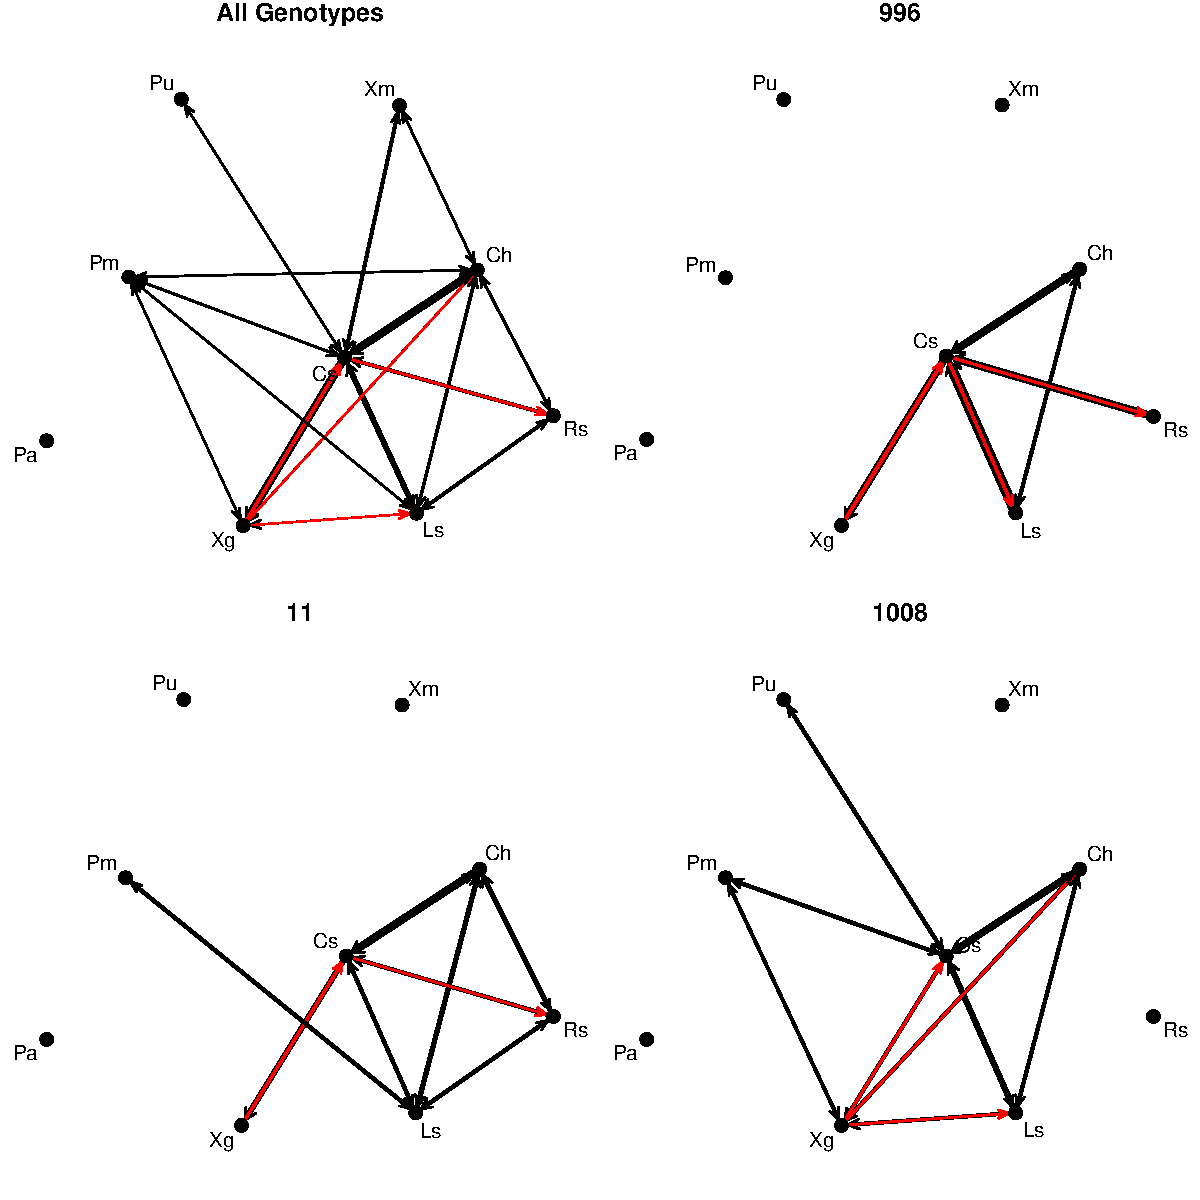
\includegraphics[width=\linewidth]{cn_onc.pdf}
\caption{}
\label{fig:cn_onc_app}
\end{figure*}

\begin{figure*}[ht]
\centering
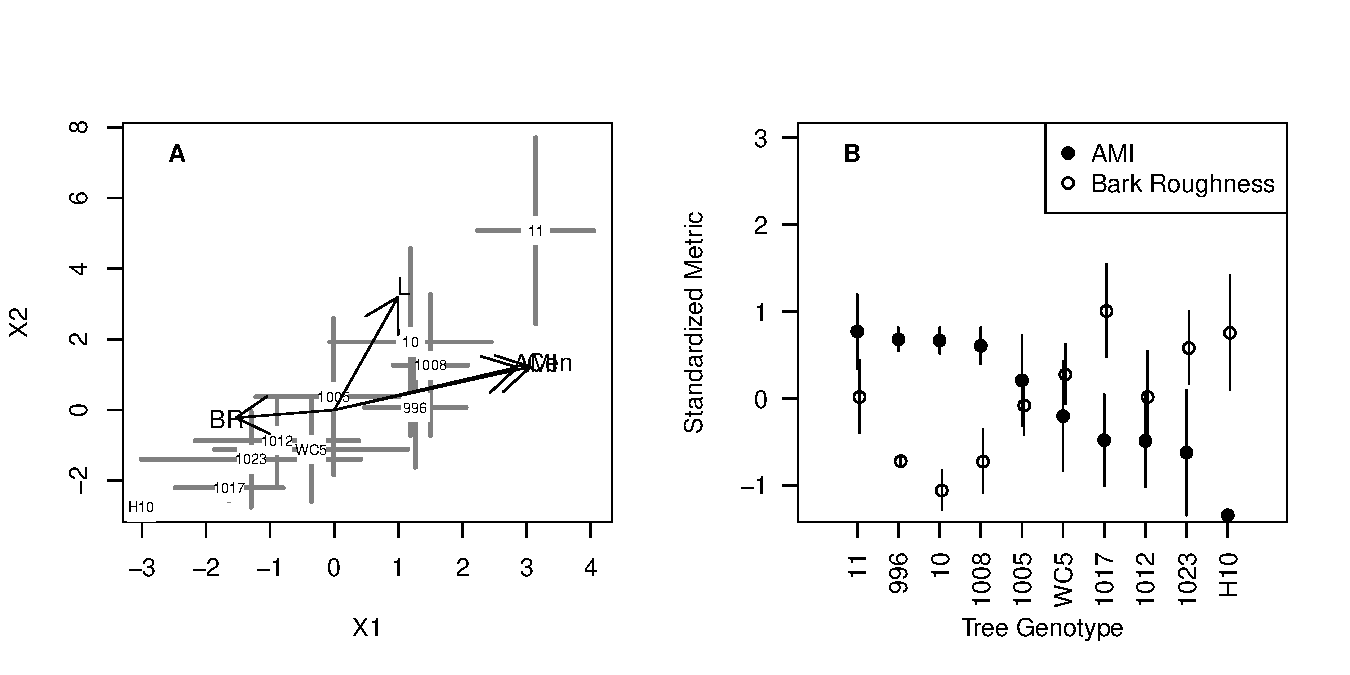
\includegraphics[width=\linewidth]{h2_plot.pdf}
\caption{}
\label{fig:h2_plot_app}
\end{figure*}

\begin{figure*}[ht]
\centering
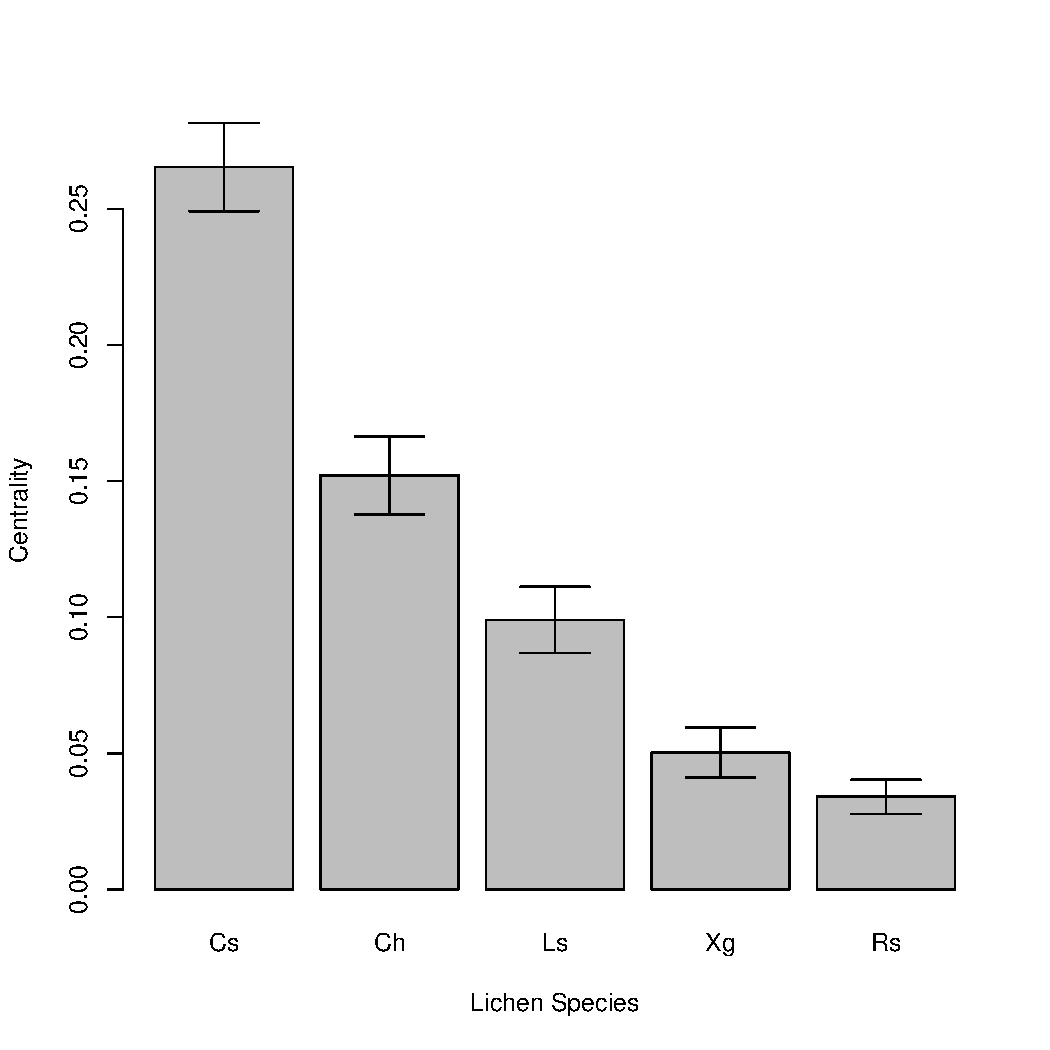
\includegraphics[width=\linewidth]{spp_cen.pdf}
\caption{}
\label{fig:spp_cen_app}
\end{figure*}

\begin{figure*}[ht]


\centering
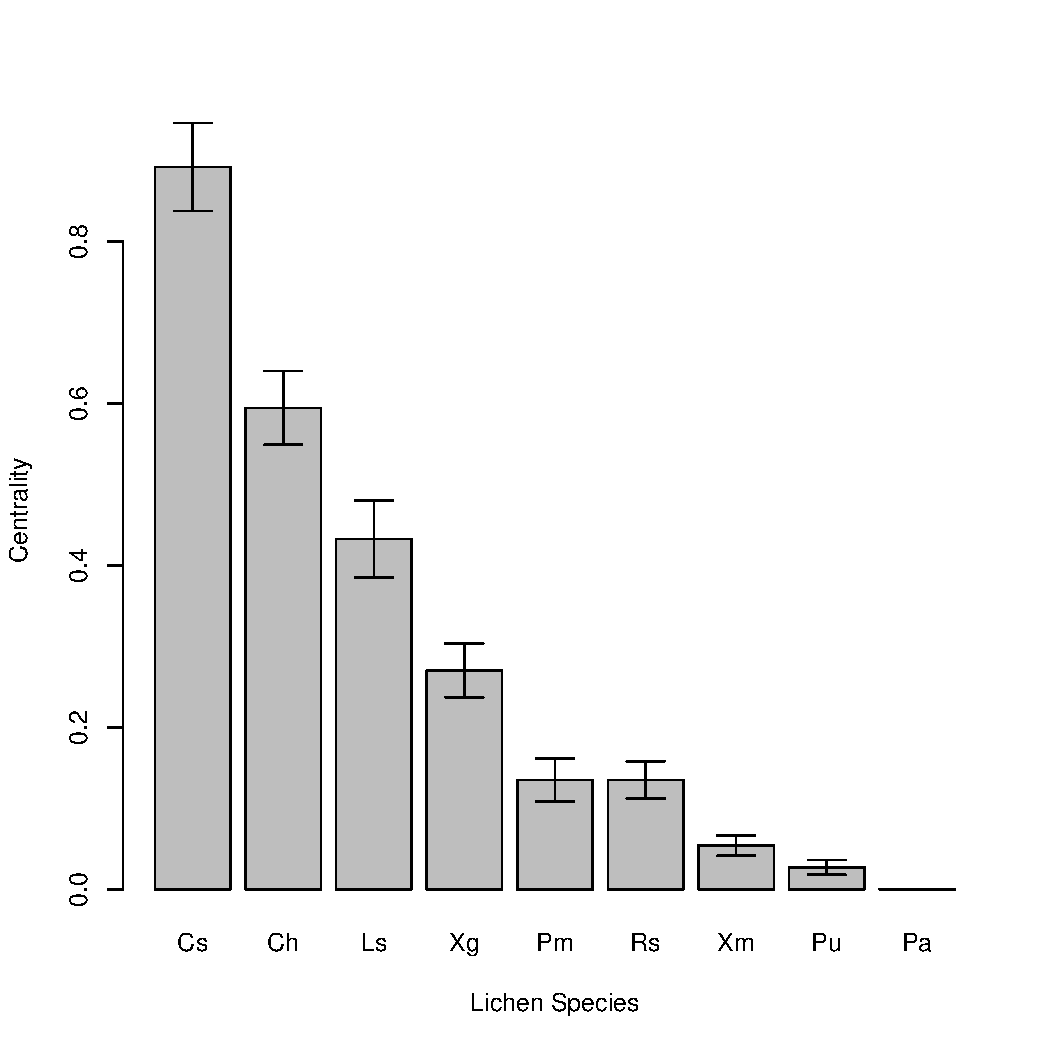
\includegraphics[width=\linewidth]{spp_cen_in.pdf}
\caption{}
\label{fig:spp_cen_in_app}
\end{figure*}

\begin{figure*}[ht]
\centering
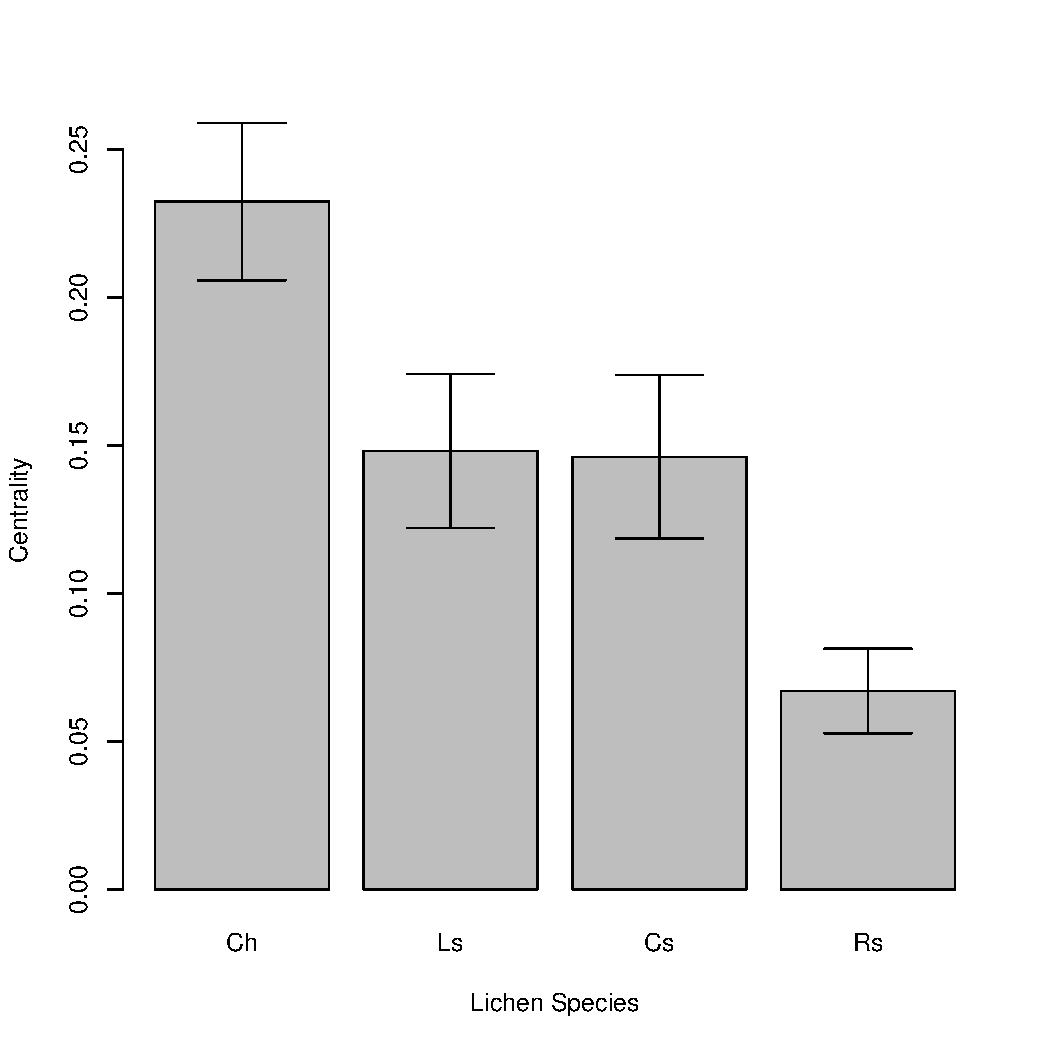
\includegraphics[width=\linewidth]{spp_cen_out.pdf}
\caption{}
\label{fig:spp_cen_out_app}
\end{figure*}

\begin{figure*}[ht]
\centering
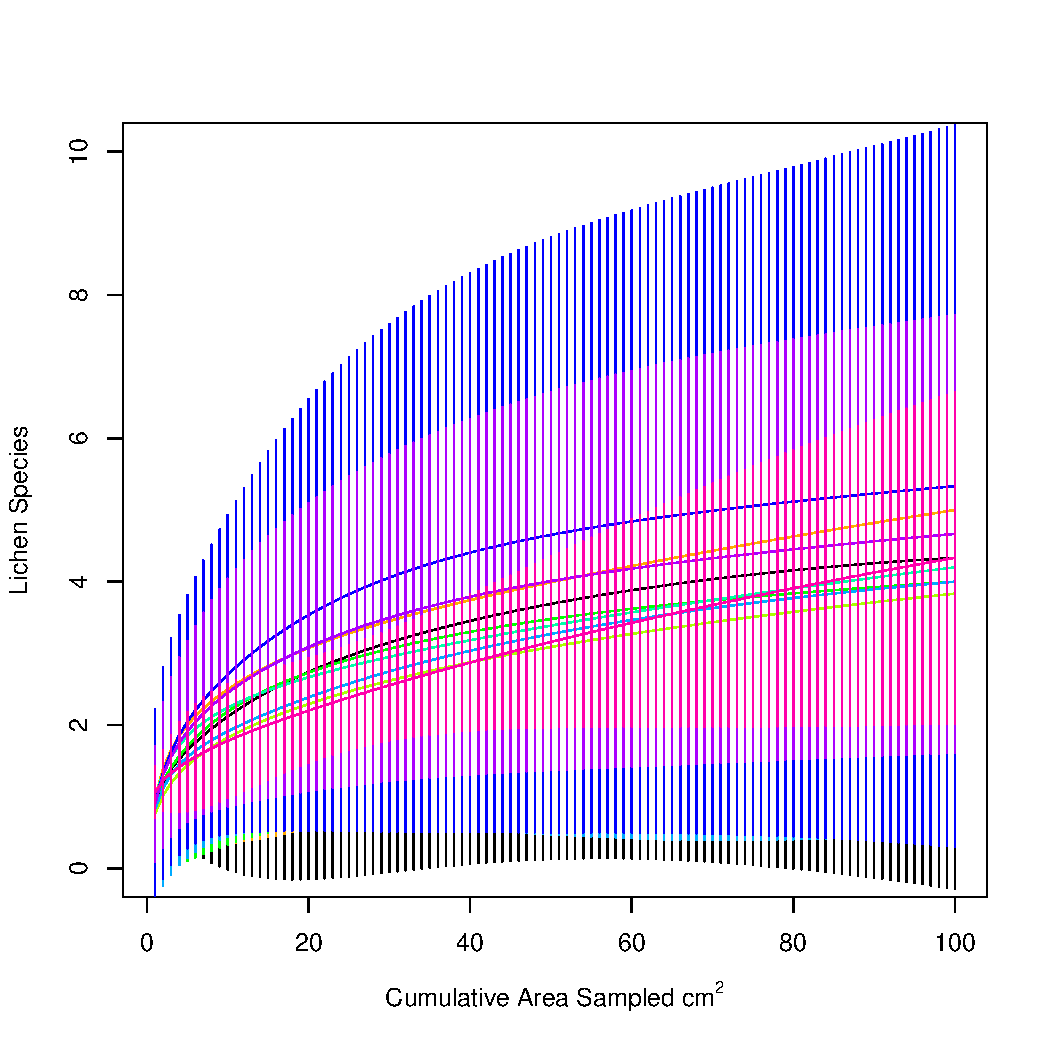
\includegraphics[width=\linewidth]{spac_geno.pdf}
\caption{Species area curve by genotype.}
\label{fig:spac_geno_app}
\end{figure*}


\begin{figure*}[ht]
\centering
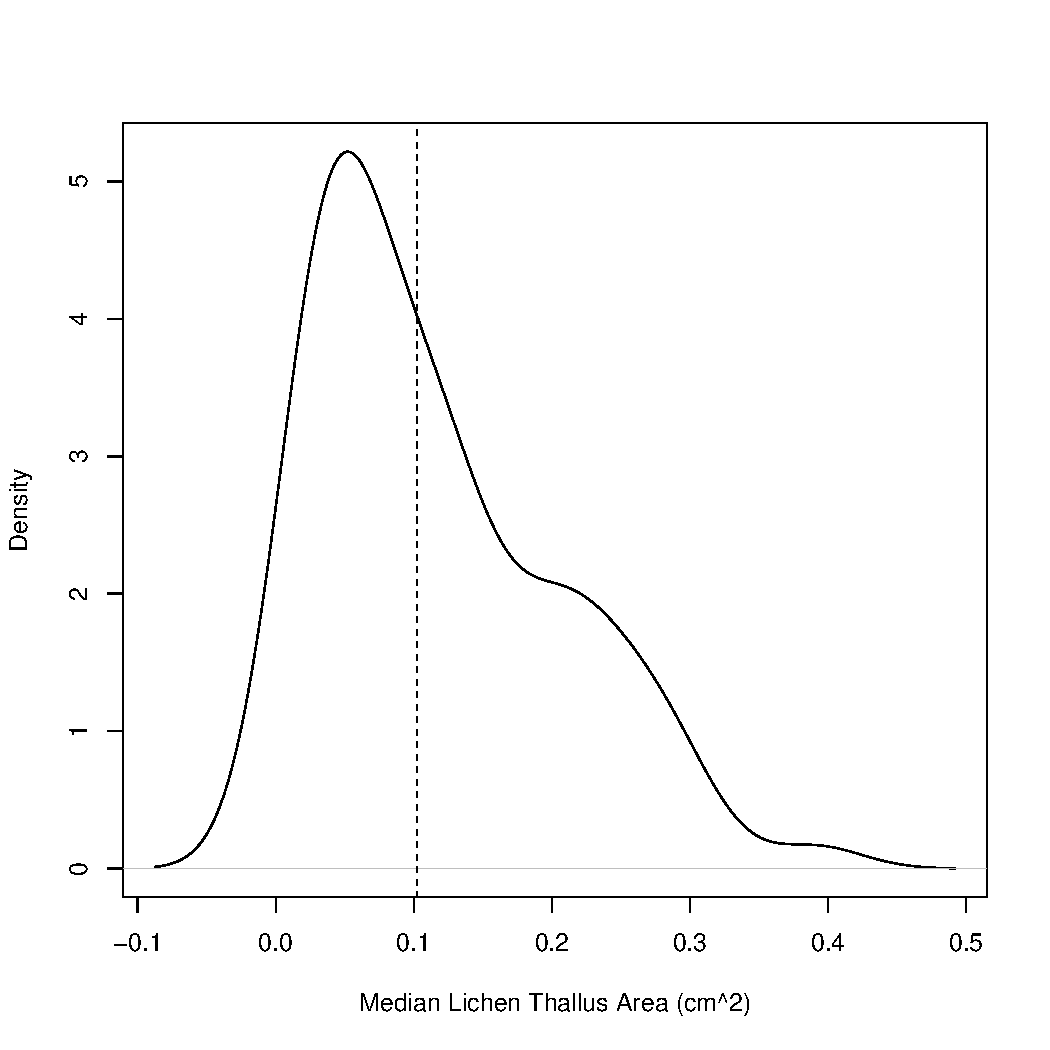
\includegraphics[width=\linewidth]{xg_size.pdf}
\caption{}
\label{fig:xg_size_app}
\end{figure*}

\end{document}

%% \subsection*{Supporting Information (SI)}

%% Authors should submit SI as a single separate PDF file, combining
%% all text, figures, tables, movie legends, and SI references.  PNAS
%% will publish SI uncomposed, as the authors have provided it.
%% Additional details can be found here:
%% \href{http://www.pnas.org/page/authors/journal-policies}{policy on
%% SI}.  For SI formatting instructions click
%% \href{https://www.pnascentral.org/cgi-bin/main.plex?form_type=display_auth_si_instructions}{here}.
%% The PNAS Overleaf SI template can be found
%% \href{https://www.overleaf.com/latex/templates/pnas-template-for-supplementary-information/wqfsfqwyjtsd}{here}.
%% Refer to the SI Appendix in the manuscript at an appropriate point
%% in the text. Number supporting figures and tables starting with S1,
%% S2, etc.

%% Authors who place detailed materials and methods in an SI Appendix
%% must provide sufficient detail in the main text methods to enable a
%% reader to follow the logic of the procedures and results and also
%% must reference the SI methods. If a paper is fundamentally a study
%% of a new method or technique, then the methods must be described
%% completely in the main text.

%% \subsubsection*{SI Datasets} 

%% Supply Excel (.xls), RTF, or PDF files. This file type will be
%% published in raw format and will not be edited or composed.

%% \subsubsection*{SI Movies}

%% Supply Audio Video Interleave (avi), Quicktime (mov), Windows Media
%% (wmv), animated GIF (gif), or MPEG files and submit a brief legend
%% for each movie in a Word or RTF file. All movies should be
%% submitted at the desired reproduction size and length. Movies
%% should be no more than 10 MB in size.


%% \subsubsection*{3D Figures}

%% Supply a composable U3D or PRC file so that it may be edited and
%% composed. Authors may submit a PDF file but please note it will be
%% published in raw format and will not be edited or composed.

